\documentclass{article}
% This text is inserted in the beginning of all
% LaTex and Tex files I create.
%
% File created: Thu Apr  1 2010
% File name:    paper.tex
% Path:         /home/mroughan/Reports/Networking/Topology/Waxman/
%
% Matthew Roughan
% matthew.roughan@adelaide.edu.au
%
\usepackage{fancyhdr}
\usepackage{epsf}
\usepackage{subfig}
\usepackage{latexsym}
\usepackage{dsfont}
\usepackage{url}
\usepackage{times}
\usepackage{graphicx}
\usepackage{amsfonts}
\usepackage{amsmath}
\usepackage{ifthen}
\usepackage{verbatim}
\usepackage{cite}
\usepackage{amsfonts}
\usepackage{amssymb}

\setlength{\headheight}{10mm}
\setlength{\headsep}{10mm}
\setlength{\topmargin}{0cm}
\setlength{\textwidth}{175mm}
\setlength{\textheight}{225mm}
\setlength{\oddsidemargin}{-10mm}
\lefthyphenmin=2
\righthyphenmin=3

\renewcommand{\baselinestretch}{1.0}
\renewcommand{\textfraction}{0.1}


% \def\RR{\mathds{R}}
% \def\CC{\mathds{C}}
\def\R{\mathbb{R}}
\def\C{\mathbb{C}}
\def\Z{\mathbb{Z}}
\def\x{{\mathbf x}}
\def\y{{\mathbf y}}

\newcommand{\titlestr}{The Line-Picking Problem}
\rhead[]{{\small \titlestr}}
\lhead[{\small }]{}
\cfoot{}
\rfoot[]{{\rm\thepage}}
\lfoot[{\rm\thepage}]{}
\renewcommand{\footrulewidth}{0.4pt}
\pagestyle{fancy}

\newtheorem{theorem}{Theorem}[section]
\newtheorem{lemma}{Lemma}[theorem]
\newtheorem{corollary}[theorem]{Corollary}
\newtheorem{Def}{Definition}[section]

\renewcommand\arraystretch{2.0} 
% \newcommand{\full}[1]{#1}
\newcommand{\full}[1]{}

\begin{document}
\title{\titlestr}
\author{Matthew Roughan \;\;\; Eric Parsonage \;\;\; Jonathan Tuke \\
 School of Mathematical Sciences \\
 University of Adelaide \\
 \url{ <{matthew.roughan,eric.parsonage,}@adelaide.edu.au> } }
\maketitle

\begin{abstract}

\end{abstract}

\section{Introduction}

The {\em line-picking} problem is a standard problem in stochastic
geometry, where we pick lines at random from some region. The typical
questions one asks are what will then mean line length be? What will
the Probability Density Function (PDF) be?

This brief note describes the current list of known PDFs, and where
they were derived, as well as the current set of code to calculate
these. 

The code is written in C with minimal external dependencies, and with
suitable wrapper functions for Matlab and R, to allow it to be run on
a wide variety of systems.



Motivation: examples of uses
\begin{itemize}

\item Modelling a PNNI hierarchical routing protocol for ATM packet
  telecommunication networks~\cite{Rosenberg200499} (length of lines
  in rectangles);

\item 

\end{itemize}

Apart from a systematic survey of the line-picking problem, we have
made several contributions in this paper:
\begin{itemize}

\item For many line-picking problems, there have been works that
  determined the Probability Density Function (PDF), or Cumulative
  Density Function (CDF), or just mean and/or variance. It should be
  clear that give either the PDF or CDF the other quantities are all
  obtainable numerically, however, we primarily focus here on
  closed-form solutions, and we have provided such for many of the
  currently absent cases, e.g., the CDF for the rectangle line-picking
  problem. 

\item We have extended the circle and sphere line-picking problems to
  the $n$-sphere.

\item We have extended the line-picking problem onto addition regions,
  in particular the cylinder, ...

\item We have extended the line-picking problem to consider different
  notions of distance: for example, the Manhattanor the $L_{\infty}$
  distance on the rectangle and n-cube

\item We have extended the line-picking problem to geodesics on
  certain surfaces, notable the cylinder and $n$-sphere.

\end{itemize}



\section{Problem Definition}

Although, commonly called the ``line-picking'' problem, the problem is
more often motivated in practical problems (such as those described
above), by the problem of finding the distance between two random
points. 

This is a much better way to describe the problem. It avoids
Bertrand's paradox, where (at least) three methods of choosing a chord
of a circle at random leads to confusion and a ``paradox''.
% http://www.sciencedirect.com/science/article/pii/S0167637703000725
% http://en.wikipedia.org/wiki/Bertrand_paradox_%28probability%29
So here we shall focus on lines determined by two IID end-points, but
we shall generalize the problem substantially to motivate by the
practical problems discussed above.

We define a {\em line-picking problem} to consists of 3 components:
\begin{itemize}

\item Some space $\Omega$ (typically a subset of $R^n$), on which we
  draw independent pairs of random points.

\item The measure $\mu$ on $\Omega$ giving the probability of drawing
  points from given segments of $\Omega$. The most common measure, by
  far, is the uniform measure, resulting in a generalized Poisson
  process of points on the $\Omega$.

\item A distance metric $D(\cdot, \cdot)$ on the space $\Omega$. One
  way to think of this is we are drawing ``lines'', i.e., geodesics,
  in some space $\Sigma$ in which $\Omega$ is embedded. The most
  common case is that the space $\Sigma = \R^n$, and the distance
  metric is simple Euclidean distance. In this case, the geodesics are
  simple lines -- hence the name of the problem. However, there are
  other possibilities.

\end{itemize}
We describe these problems by the triple: $\big(\Omega, \mu, D(\cdot,
\cdot)\big)$. However, the common cases are so common that we ommit
mentioning that the measure is uniform, or that the distance metric is
Given that the typical case of $\mu$ is uniform, and of $d$ is
Euclidean, we ommit these from the problem statement when we use these
simple defaults.

Figure~\ref{fig:eg} presents three examples: the disk-line-picking
problem, the circle-line-picking problem and the cube-line-picking
problem.

\begin{figure}[tbp]
% Figures generated with ../Matlab/Examples/LinePicking_eg.m
  \begin{center}
    \subfloat[\label{fig:disk_eg}Disk-line-picking.]%
          {\includegraphics[width=0.33\columnwidth]{../Matlab/Plots/LinePicking_eg_disk.eps}}
    \subfloat[\label{fig:circle_eg}Circle-line-picking.]%
          {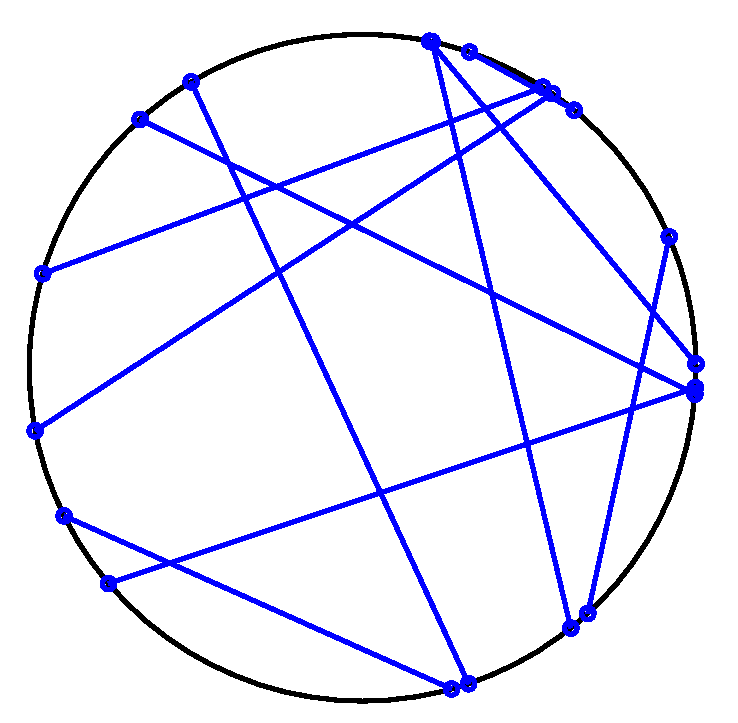
\includegraphics[width=0.33\columnwidth]{../Matlab/Plots/LinePicking_eg_circle.eps}}
    \subfloat[\label{fig:cube_eg}Cube-line-picking.]%
          {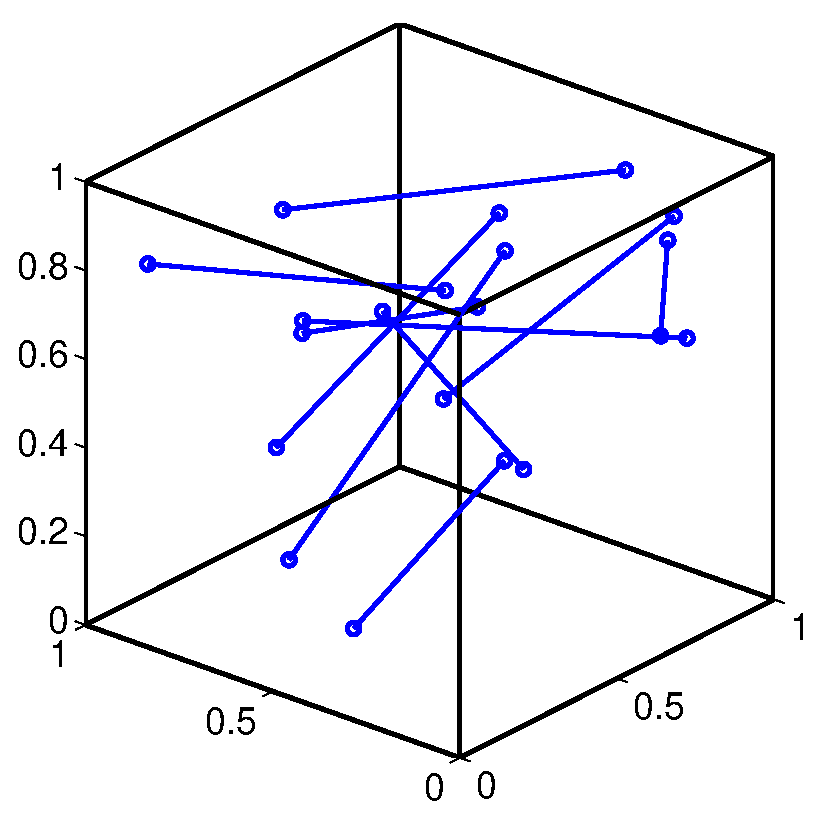
\includegraphics[width=0.33\columnwidth]{../Matlab/Plots/LinePicking_eg_cube.eps}}
    \caption{Example line-picking problems.\label{fig:eg}}
  \end{center} 
\vspace{-4mm}
\end{figure}


\section{General Properties}
\label{sec:general}

\begin{enumerate}

\item Most of the cases are defined over finite regions, and hence the
  PDFs have finite support.

\item All of the distributions are {\em proper}

\item Almost all are defined on continuous, convex sets, and in this
  case the distributions are continuous, i.e., the CDF is a continuous
  function.

\item Almost all are defined on continuous, convex sets, and in this
  case the PDFs are also continuous functions.

\end{enumerate}

\subsection{Region Transforms}
\label{sec:scaling}

Many of the standard problems use a uniform point distribution and
Euclidean distances on some convex region of $R^n$. In these cases,
there is are easy scaling and trasnlation laws that means once we know
the distribution for some size region, we can compute it for any size.

Translation is trivial. Given the uniform distribution of point,
translation has no affect on the line-length distribution.

Scaling is almost as simple: if the region $\Omega$ is scaled in all
dimensions by $L$, then the problem is identical under a scaling of
the distance metric by $L$. We can therefore scale the density
functions as follows
\begin{equation}
   g_L(t) = \frac{1}{L} g_1 \left( \frac{t}{L} \right). 
\end{equation}
Non-uniform scaling is not so simple as we shall see in the results
below.

Scaling for CDFs is even simpler, we simply take
\begin{equation}
   G_L(t) = G_1 \left( \frac{t}{L} \right). 
\end{equation}


\section{Cartesian products of spaces}

One of the aspects of the line-picking problem that doesn't seem
generally considered is how to derive results for constructed
space. Perhaps the simplest example of which is the Cartesian product
of two spaces.

The Cartesian product is defined by
\begin{equation}
 S \times T = \{ (s,t) | s \in S, t \in T \}. 
\end{equation}
For instance, the square, which is the Cartesian product of two lines
segments, has been as extensively considered as any line-picking
problem, but this basic constructivist approach is not used, except
implicitly. 

The useful feature of the Cartesian product is that if we take two
independent random variables $X \in S$ and $Y \in T$, each uniformly
distributed over their respective spaces, then the random varible
$(X,Y)$ will be uniformly distributed over the space $S \times T$. As
a result, we easily can construct uniformly distributed points from
these component spaces. 

The reason it is interesting is because we can construct many common
example from Cartesian products. It also helps us to extend the notion
of the line-picking problem to spaces with alternative metrics, and
even combined metrics. For instance, assume we have distance metric
$d_S$ on $S$ and $d_T$ on $T$, we can form a new distance metric on $S
\times T$ by taking
\begin{equation}
  d_{S \times T}\Big( (X_1,Y_1), (X_2,Y_2)  \Big)
 = \left\{ \begin{array}{ll}
      \sqrt{ d_S(X_1,X_2)^2 +  d_T(Y_1,Y_2)^2}, \\
      | d_S(X_1,X_2) +  d_T(Y_1,Y_2)|, \\
      \max\{ d_S(X_1,X_2) +  d_T(Y_1,Y_2) \}, \\
    \end{array}
  \right.
\end{equation}
for the Euclidean, $\ell_1$ and $\ell_{\infty}$ distances,
respectively (though note that there is no real requirement that the
distances $d_S$ and $d_T$ match, or that they match the combining
operation, in order to create a valid metric. Moreover, there are some
interesting cases where they don't match.

Given we know the distribution of the distances on $S$ and $T$, we
should therefore be able to construct statistics for the distance
distribution on the product space, without deriving this from first
principles. We do so below for each of these cases. However, the order
in which we derive information (e.g., PDFs, CDFs, moments, etc.) may
vary depending on the metric, so we consider each below separately. 

\subsection{The Euclidean metric}

The classic Euclidean distance metric is actually one of the hardest
to work with, but there are several useful results.

The even moments $2k$ expand into a binomial, and we can exploit this
to derive formulae for the moments in terms of the moments of the
component spaces. For instance, given distances $X$ and $Y$ in each
space, then $X^2$ and $Y^2$ are independent random variables, and so
\begin{eqnarray}
  E\left[ \left( \sqrt{ X^2 + Y^2} \right)^{2k} \right] 
   & = & \sum_{i=0}^{k} \dbinom{k}{i} E[X^{2i}] E[Y^{2(n-i)}].
\end{eqnarray}



% In general we can compute 
% However, the odd moments are more difficult. 
% \begin{eqnarray}
%   E\left[ \left( \sqrt{ X^2 + Y^2} \right)^{2n+1} \right] 
%    & = &  \sum_{k=0}^{\infty}  \dbinom{(2n+1)/2}{k} E[X^{2k}] E[Y^{2n+1-2k}].
% \end{eqnarray}
% -- but  this may not work because of convergence?



We can also derive useful relationships for the PDF in the same
way. As above, it is  to work with squared distances, which will have
PDFs 
\begin{eqnarray}
  \label{eq:h_g}
  h_{X^2}(u) & = & g_X(\sqrt{u})/(2\sqrt{u}), \\
  h_{Y^2}(u) & = & g_Y(\sqrt{u})/(2\sqrt{u}), \\
\end{eqnarray}
The PDF for the sum of independent random variables is
obtained by taking the convolution of their PDFs, and we can see that
the squared distances add here, so
\begin{eqnarray}
  \label{eq:add_euclidean}
  h_{X^2+y^2}(u) & = & \int_{-\infty}^\infty h_{X^2}(s)  h_{Y^2}(u-s) \, ds
\end{eqnarray}
This convolution can then be computed directly, or by taking Laplace
tranforms (and noting that this results in a product in the Laplace
domain).  The chief difficulty in computing this convolution is often
simply that the support for most of the PDFs considered here is
finite, and therefore, the integral often breaks into different
pieces.

We can then transform back to obtain the PDF of the actual distances
by noting that
\begin{equation}
  \label{eq:g_h}
  g_{\sqrt{X^2+Y^2}}(t) 
     =  2 t \, h_{X^2+y^2}(t^2).
\end{equation}

If it is easier to compute this directly, then it may be easier to
compute moments by integrating the PDF, rather than integrating
variables directly, or using other techniques describe above.


\subsection{Manhattan distance}

In the case of the Manhattan distance, i.e., where we combine
submetrics using the sub of their absolute values, we can note that
the submetrics are guaranteed to be non-negative, and hence we are
simply adding independent random variables. Hence computing the
moments is almost trivial, i.e., 
\begin{eqnarray}
  E\left[ \left( X + Y \right)^{k} \right] 
   & = & \sum_{i=0}^{k} \dbinom{k}{i} E[X^{i}] E[Y^{(n-i)}].
\end{eqnarray}
The cross-terms of the second central moment cancel, and so the mean
and variance are simply the sum of the mean and variance of the
relevant submoments.

We can construct the PDF using convolutions as above, though without
the transforms between squared variables and back, or we could
construct them (at least numerically) by using the above moment
construction, and then inverting the moment generating function:

....


\subsection{Max metric}

When working with the maxx-metric, there is no simple relationship
between moments of the Cartesian product and its components. However,
the CDF is almost trivial to construct, as it is simply given by
\begin{equation}
  \label{eq:cdf_construction}
  G_{\max\{X,Y\}}(t)
    = \mbox{Prob}\{ \max\{X,Y\} \leq t \}
    = \mbox{Prob}\{ X \leq t \mbox{ and } Y \leq t \}
    = \mbox{Prob}\{ X \leq t \} \times \mbox{Prob}\{ Y \leq t \}
    = G_X(t) G_Y(t). 
\end{equation}


For the Max distance, there is no simple relationship, but the
simplicity of computing the PDF and CDF mean that computing the
moments is often not hard.



\section{Examples}
\label{sec:known}

We go through a list of examples, some from the literature, and some
derived here, though derivations are typically delayed until the
appendices in order to make the flow easy.

\begin{figure}[htbp]
  \begin{center}
% Figures generated with ../Matlab/Examples/LinePicking_plot.m
    \includegraphics[width=0.5\columnwidth]{../Matlab/Plots/LinePicking_plot_fix_area.eps}

    \label{fig:various}
    \caption{Example distance densities for shapes with area fixed to 1.}
  \end{center} 
\vspace{-4mm}
\end{figure}


\clearpage
\subsection{Line-line picking}
\label{sec:line_line}


\subsubsection{PDF}

The probability density function of distances between two (uniformly)
randomly chosen points on the unit line is given in
\cite{weisstein:_line_line_picking,b.ghosh51:_random_rect}, as
\begin{equation}
  \label{eq:line_line}
  g^{\rm line}(t) = 2(1-t),
\end{equation}
or for a line of length $L$ as
\begin{equation}
  \label{eq:line_lineL}
  g^{\rm line}_L(t) = \frac{2}{L} \left( 1-\frac{t}{L} \right).
\end{equation}

This also arises as the limit as $a \rightarrow 0$ for the PDF for the
rectangle \eqref{eqn:rectangle}.

\subsubsection{CDF}


\subsubsection{Moments}






\clearpage
\subsection{Square-line picking}
\label{sec:square_line}

Here we consider choosing lines from a unit square, where the
end-points are chosen IID uniformly from the unit
square. Figure~\ref{fig:square_eg} shows a simple example.

This is an obvious special case of the rectangle, but we consider it
here separately because the results are somewhat simpler, and hence
more intuitive. Also, as this is a special case of the rectangle, it
provides a useful check as to the accuracy of the implementation of
both formula. However, for that reason, we only bother to present the
results for the unit square here.

The PDF is shown in Figures~\ref{fig:square_pdf}, which uses different
coloured shading to highlight the two regions, and the continuity of
the PDF at the boundary. Table~\ref{tab:summary_line} shows the basic
statistics for the unit-square line picking problem.

\begin{figure}[htbp]
  \begin{center}
    \subfloat[\label{fig:square_eg}Example.]
       {\includegraphics[width=0.35\columnwidth]{../Matlab/Plots/LinePicking_eg_square.eps}} 
    \hspace{3mm}
    \subfloat[\label{fig:square_pdf}PDF.]
       {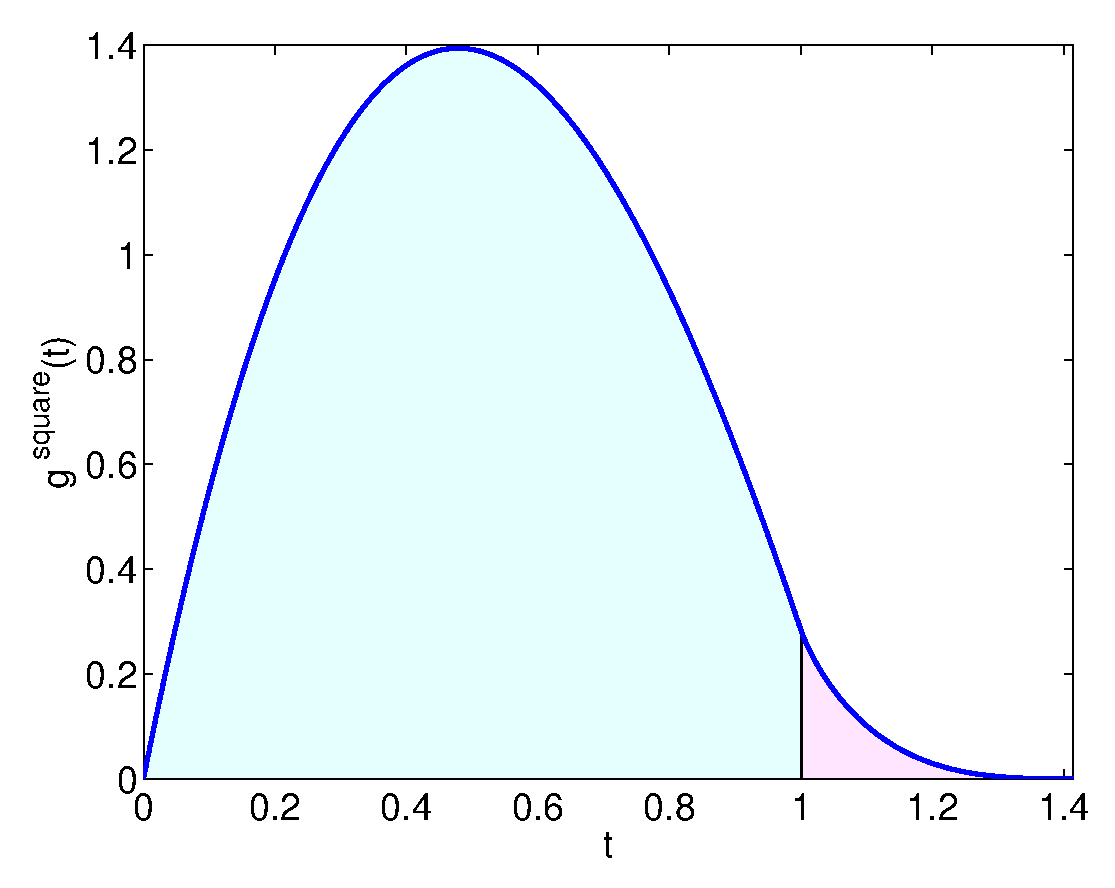
\includegraphics[width=0.4\columnwidth]{../Matlab/Plots/LinePicking_plot_square_pdf.eps}}
    \caption{The unit-square line-picking problem.}
  \end{center} 
\vspace{-4mm}
\end{figure}

\begin{table}[ht]
  \centering
  \begin{tabular}{|r|c|l|}
    \hline
    Statistic & Value & Source \\ 
    \hline
      PDF                & $\displaystyle 
  g^{\rm square}(t) = \left\{ \begin{array}{ll}
      2t (t^2-4t+\pi),
               & \mbox{ for } 0 \leq t \leq 1, \\
      2t \left[4 \sqrt{t^2-1} - (t^2+2-\pi) - 4 \tan^{-1} \left(\sqrt{t^2-1} \right)\right], 
               & \mbox{ for } 1 \leq t \leq \sqrt{2} . \\ 
    \end{array} \right.
                                 $ &
                             \cite{philip:_probab_distr_distan_between_two,weisstein:_squar_line_picking} \\
      CDF                & $\displaystyle
  G^{\rm square}(t) = \left\{ \begin{array}{ll}
      \frac{1}{2} t^4 - \frac{8}{3} t^3 + \pi t^2, 
               & \mbox{ for } 0 \leq t \leq 1, \\
      -\frac{1}{2} t^4 + (\pi-2)t^2 + \frac{1}{3}
                   +\frac{4}{3} \left( 2t^2+1 \right)\sqrt{t^2-1} 
                     & \\
                   \hspace{12mm} - 4 t^2 \tan^{-1} \left(\sqrt{t^2-1} \right),
               & \mbox{ for } 1 \leq t \leq \sqrt{2} . \\ 
    \end{array} \right.
                                 $ & 
                             \cite{weisstein:_squar_line_picking} \\
      $i$th Moment $m_i$ & $\displaystyle 
                                 $ &
                              \cite{weisstein:_squar_line_picking} \\
      Mean               & $\displaystyle \frac{2 \sqrt{2} + 5\sinh^{-1}(1)}{15}
                             = 0.521405433...$ &
                             \cite{weisstein:_squar_line_picking} \\
      Variance           & $\displaystyle \frac{}{225}
                             = 0.061469...$ &
                             \cite{weisstein:_squar_line_picking} \\[1.5ex]
    \hline
  \end{tabular}
  \caption{Summary of the line-line picking problem for a line of
    length $L$.}
  \label{tab:summary_line}
\end{table}

\subsubsection{PDF}

The PDF for the unit square is given in
\cite{philip:_probab_distr_distan_between_two,weisstein:_squar_line_picking},
but which
\begin{equation}
  \label{eq:square_line}
  g^{\rm square}(t) = \left\{ \begin{array}{ll}
      2t (t^2-4t+\pi), & \mbox{ for } 0 \leq t \leq 1, \\
      2t \left[4 \sqrt{t^2-1} - (t^2+2-\pi) - 4 \tan^{-1} \left(\sqrt{t^2-1} \right)\right], 
               & \mbox{ for } 1 \leq t \leq \sqrt{2} . \\ 
    \end{array} \right.
\end{equation}
% http://mathworld.wolfram.com/SquareLinePicking.html

Generalization to larger squares can be done by scaling (see
Section~\ref{sec:scaling}), or by using the rectangle-line pick1ing
solution (see Section~\ref{sec:rectangle_line}).


 is also a special case of the PDF for the rectangle
\eqref{eqn:rectangle} with $a=b$.

\subsubsection{CDF}


\subsubsection{Moments}



\subsubsection{Related Problems}

A related problem we don't include here (at the moment) is the problem
of choosing two points on two (different) edges of a square.

\url{http://oeis.org/A091506}

D. H. Bailey, J. M. Borwein, V. Kapoor and E. Weisstein, Ten Problems
in Experimental Mathematics

average distance is $(2 + sqrt(2) + 5*ArcSinh[1])/9$



\clearpage
\subsection{Rectangle-line picking}
\label{sec:rectangle_line}


Here we consider choosingp lines from a rectangle with side lengths
$a$ and $b$, which we order $a \leq b$ without loss of generality. 
We could also describe the problem by the aspect ratio of the
rectangle, i.e., $a \!: \!b$.

Figure~\ref{fig:rect_eg} shows a 2D example, Figure~\ref{fig:rect_pdf}
shows the PDF for one rectangle, and Figure~\ref{fig:rect_pdf_var}
shows the PDFs for various rectangles chosen such that $\sqrt{a^2 +
  b^2} = 1$ to allow comparison (the choice means that the PDFs have
the same support).

\begin{figure}[tbp]
  \begin{center}
    \subfloat[\label{fig:rect_eg}Rectangle example.]{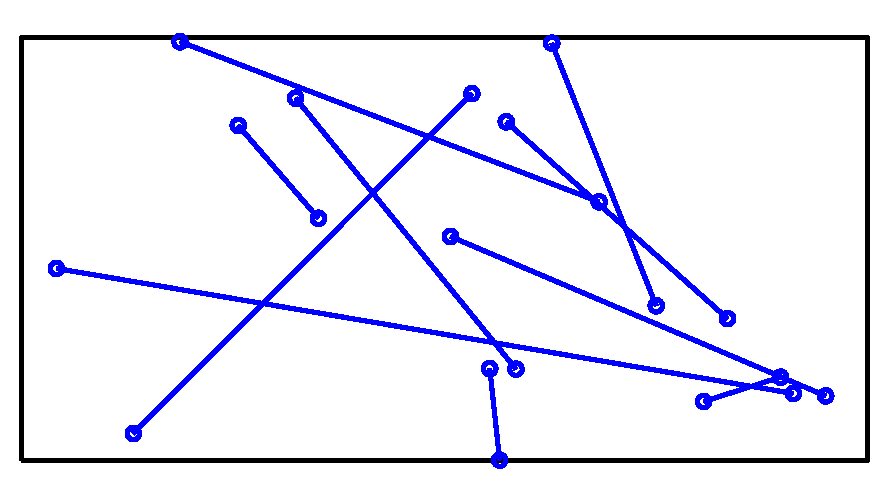
\includegraphics[width=0.28\columnwidth]
          {../Matlab/Plots/LinePicking_eg_rect.eps}} 
    \hspace{6mm}
    \subfloat[\label{fig:rect_pdf}PDF of a rectangles with aspect
    ratio 1:1.2 showing the three regions.]{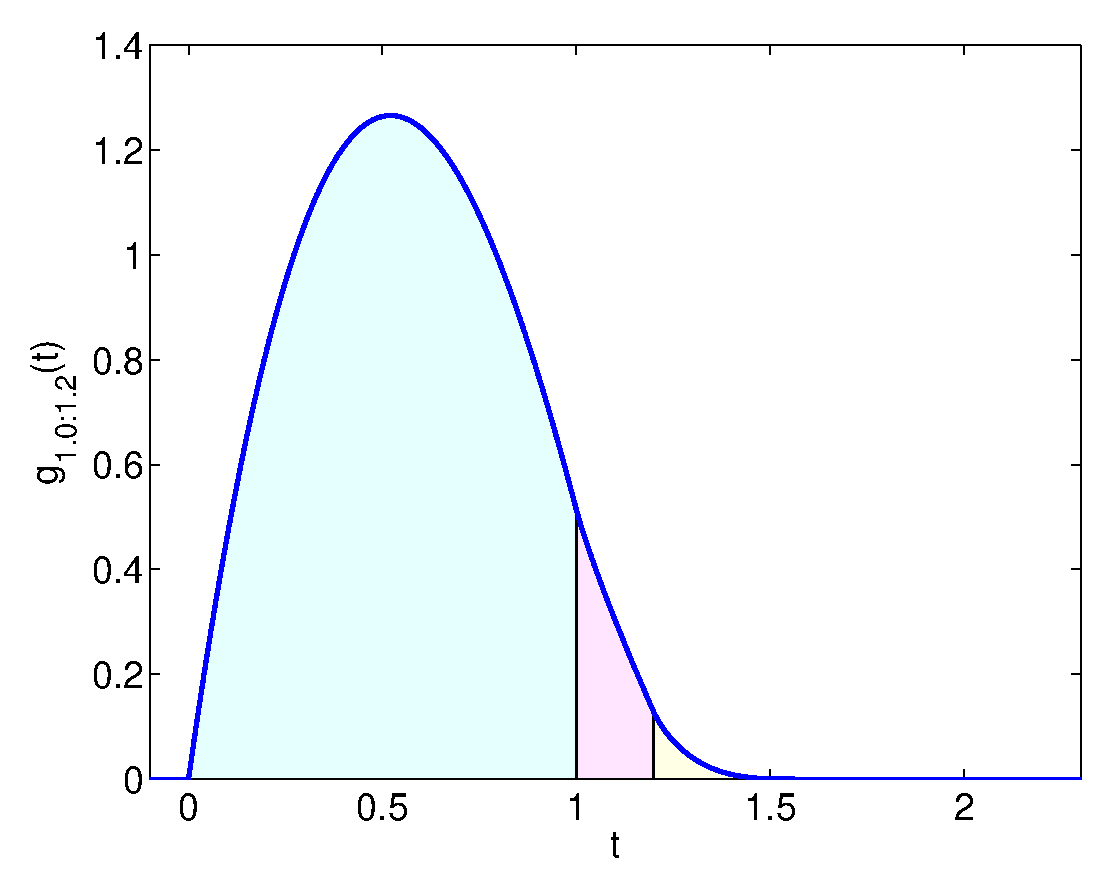
\includegraphics[width=0.35\columnwidth]
          {../Matlab/Plots/LinePicking_plot_rect_regions.eps}}
    \subfloat[\label{fig:rect_pdf_var}PDF of rectangles with various aspect
    ratios.]{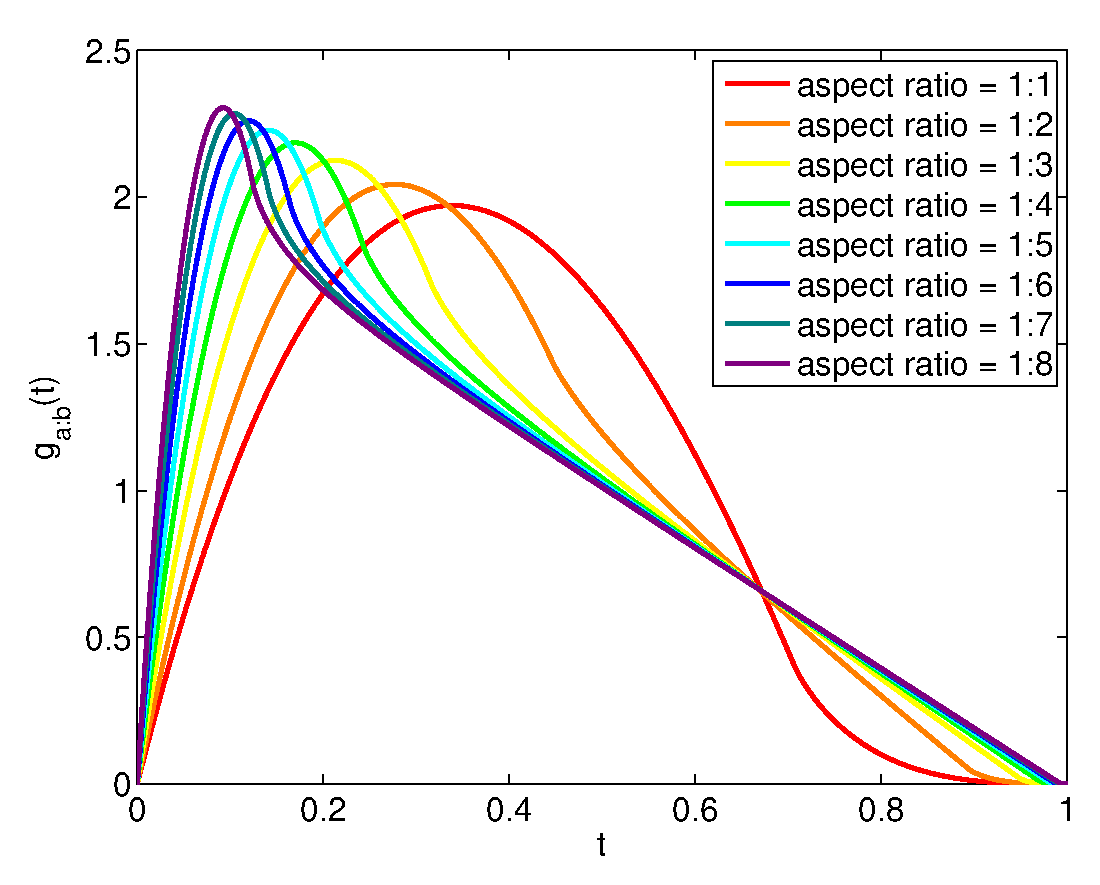
\includegraphics[width=0.35\columnwidth]
          {../Matlab/Plots/LinePicking_plot_rect.eps}}
    \caption{The rectangle-line picking problem.}
  \end{center} 
\vspace{-4mm}
\end{figure}

\subsubsection{PDF}

The PDF for the rectangle is given in \cite[Theorem
2.4.4]{mathai_geom} and \cite[Theorem 2]{b.ghosh51:_random_rect}
\begin{equation}
  g^{\rm rect}_{a,b}(t) = \frac{4 t}{a^2 b^2} \phi_{a,b}(t),
  \label{eqn:rectangle}   
\end{equation}
where
\begin{equation}
  \phi_{a,b}(t) = \left\{
    \begin{array}{ll}
      \frac{ab \pi}{2} - (a+b) t + \frac{t^2}{2}, 
         & \mbox{ for } t \leq a, \\
      a b \sin^{-1} (a/t) - \frac{a^2}{2} - b t + b\sqrt{t^2 - a^2},
         & \mbox{ for } a \leq t \leq b, \\
      a b \left[ \sin^{-1} (a/t) - \sin^{-1} \sqrt{1 - \frac{b^2}{t^2}} \right]
        - \frac{a^2 + b^2 + t^2}{2} 
        + a\sqrt{t^2 - b^2}+ b\sqrt{t^2 - a^2},
         & \mbox{ for } b \leq t \leq \sqrt{a^2 + b^2}, \\
      0,
         & \mbox{ otherwise}, \\
    \end{array} \right. 
\end{equation}
where the rectangle has sides of length $a \leq
b$. Figure~\ref{fig:rect_pdf} shows these for various cases, chosen
such that $\sqrt{a^2 + b^2} = 1$ to allow comparison. We label these
rectangles by their aspect ratio $a: b$.

This is a rather complicated expression, but is easily evaluated
numerically.  Naldi \cite{m.naldi05:_connec_of_waxman_graph}
approximated this expression with a $\beta$ function, though given the
requirements to numerically evaluate that function there hardly seems
any advantage, though we shall see later that this would have been
completely appropriate if the region have been a circle.

We can also see that for longer, thinner rectangles, the PDF is
comprised of two main segments: (i) a part approximating the shape of
that for the square (though compressed into a short range of values of
$t$), and (ii) an almost straight component, similar to the PDF for
line-line picking problem. The reasons for this also seem relatively
intuitive. 

We can calculate the limit as $a \rightarrow 0$ to see the PDF for the
line-line picking problem.  We keep $a^2 + b^2 = L^2$ so that the
support of the PDF remains constant.  As $a \rightarrow 0$, we only
need consider the case $a \leq t \leq b$, where
\begin{eqnarray}
    g^{\rm rect}_{a,b}(t)
        & = & \frac{4 t}{a^2 b^2} 
                  \left[ a b \sin^{-1} (a/t) - \frac{a^2}{2} - b t + b\sqrt{t^2 - a^2} \right] , \nonumber \\
        & \simeq & \frac{4t }{a b} \sin^{-1} (a/t)
                   - \frac{2 t}{b^2}
                    + \frac{4 t}{a^2 b^2} \left[ -b t + b t - \frac{b a^2}{2 t} \right] , \nonumber \\
        & \simeq & \frac{2}{b}
                   - \frac{2 t}{b^2}, 
\end{eqnarray}
where we have used the following Taylor series around $x=0$, dropping
the higher order terms:
\[ \sin^{-1}(x) = x + \frac{x^3}{6} + \cdots, 
   \mbox{ and }
   \sqrt{t^2 - x^2} = t - \frac{x^2}{2t} - \frac{x^4}{8 t^3} \cdots .
\]
The result just returns to the line-line picking PDF.

\subsubsection{CDF}


\subsubsection{Moments}

Ghosh \cite{b.ghosh51:_random_rect} gives the first four moments of
the line-length distribution for the rectangle.
\begin{eqnarray}
  \label{eq:rect_moments} 
  \alpha_1 & = & \frac{1}{6} \left[ 
                        \frac{b^2}{a} \cosh^{-1}\left( M/b \right) +
                        \frac{a^2}{b} \cosh^{-1}\left( M/a \right) 
                 \right]
                  + \frac{1}{15} \left[ \frac{a^3}{b^2} + \frac{b^3}{a^2} \right]
                  - \frac{M}{15} \left[ \frac{a^2}{b^2} + \frac{b^2}{a^2} -3 \right],
\\
  \alpha_2 & = & \frac{1}{6} M^2, \\
  \alpha_3 & = & \frac{1}{20} \left[ 
                        \frac{b^4}{a} \cosh^{-1}\left( M/b \right) +
                        \frac{a^4}{b} \cosh^{-1}\left( M/a \right) 
                 \right]
                  + \frac{2}{105} \left[ \frac{a^5}{b^2} + \frac{b^5}{a^2} \right]
                  - \frac{2M}{105} \left[ \frac{a^4}{b^2} + \frac{b^4}{a^2}\right]
                        - \frac{5}{84} M^3, 
\\
  \alpha_4 & = & \frac{1}{15} a^4 + \frac{1}{18} a^2 b^2 + \frac{1}{15} b^4,
\end{eqnarray}
where $M = \sqrt{a^2 + b^2}$, from which we can derive the special
cases of the square and line (though these can also be derived
directly). Obviously central moments such as mean, and variance, etc.,
can be derived from these. 


\clearpage
\subsection{Line picking on the rectangle with the Manhattan distance}
\label{sec:rect_manhattan}

Example showing a different distance metric: 

% \begin{figure}[tbp]
%   \begin{center}
%     \subfloat[\label{fig:hyperball_pdf}PDF of length 1 line showing
%     exact and simulated values.]{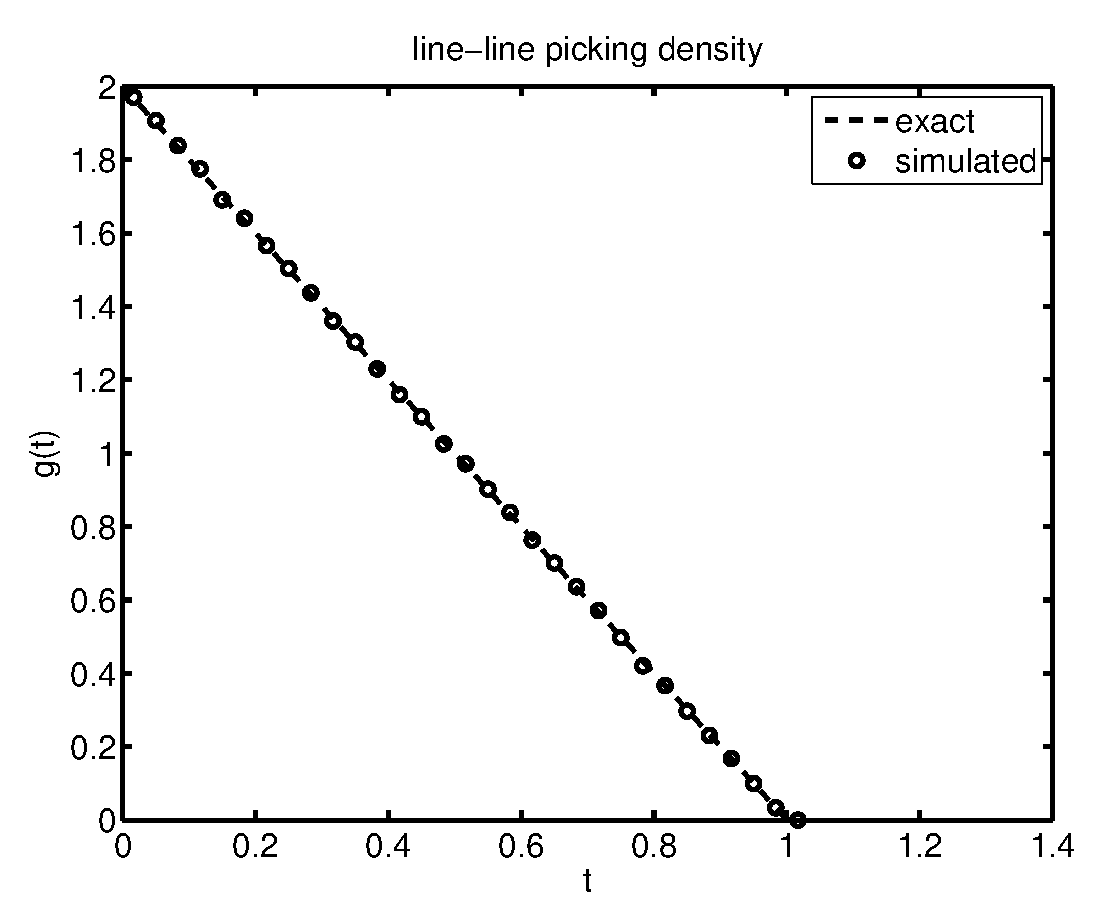
\includegraphics[width=0.48\columnwidth]{../Matlab/Plots/LinePicking_test_sim_line.eps}}
%     \caption{The line-line picking problem ($L=1$).}
%   \end{center} 
% \vspace{-4mm}
% \end{figure}

\subsubsection{PDF}

The elegant feature of this problem is that the Manhattan distance is
made up from the horizontal distance, and the vertical distance, and
these two are independent. Hence the total distance is the sum of two
independent random variables, i.e.,
\[ t_{\rm Manhattan} = t_X + t_Y, \]
where $t_X$ and $t_Y$ are distances given by the line-line picking
problem (Section~\ref{sec:line_line}).


The probability density function of distances between two (uniformly)
randomly chosen points on the unit line is given in
\eqref{eq:line_lineL}, and so the densities in the $X$ and $Y$
directions for a rectangle with sides $a$ and $b$ will be
\begin{eqnarray}
  \label{eq:rect_xy}
  g^{\rm X}_b(t) & = & \left\{ \begin{array}{ll}
                    \frac{2}{b} \left( 1-\frac{t}{b} \right), &
                         \mbox{ for } 0 \leq t \leq b, \\
                    0, & \mbox{ otherwise}, \\
                  \end{array} \right. \nonumber \\
  g^{\rm Y}_a(t) & = & \left\{ \begin{array}{ll}
                    \frac{2}{a} \left( 1-\frac{t}{a} \right), &
                         \mbox{ for } 0 \leq t \leq a, \\
                    0, & \mbox{ otherwise}. \\
                  \end{array} \right. \nonumber 
\end{eqnarray}
The density for the Manhattan distance will be the convolution of
these, i.e., for $0 \leq t \leq a+b$, and $a \leq b$, we get
\begin{eqnarray}
    g^{\rm X+Y}_b(t) & = & g^{\rm X+Y}_b(t), \nonumber \\
       & = & \left[ g^{\rm Y}_a *  g^{\rm X}_b \right] (t) \nonumber \\
       & = & \int_{-\infty}^{\infty} g^{\rm Y}_a(s)  \, g^{\rm X}_b(t-s) \, ds,  \nonumber \\
       & = & \int_{\max(0,t-b)}^{\min(a,t)} g^{\rm Y}_a(s)  \, g^{\rm X}_b(t-s) \, ds,  \nonumber \\
       & = & \frac{4}{a b} \int_{\max(0,t-b)}^{\min(a,t)}  
              \left( 1-\frac{s}{a} \right) 
              \left( 1-\frac{t-s}{b} \right)  \, ds,  \nonumber \\
       & = & \frac{4}{a b} \int_{\max(0,t-b)}^{\min(a,t)} 
                   \left( 1 - \frac{t}{b} \right)  
                    + \left( \frac{1}{b} - \frac{1}{a} + \frac{t}{a b} \right)  s  
                    - \frac{1}{a b}  s^2 
                \, ds,  \nonumber \\
       & = & \frac{4}{a b} \left[ \left( 1 - \frac{t}{b} \right) s
              + \frac{1}{2} \left( \frac{1}{b} - \frac{1}{a} + \frac{t}{a b} \right)  s^2 
              - \frac{1}{3} \frac{1}{a b}  s^3
                  \right]_{\max(0,t-b)}^{\min(a,t)},  \nonumber \\
       & = & \left\{ \begin{array}{ll}
           \displaystyle
           \frac{4}{a b} \left( 1 - \frac{t}{b} \right) t
              + \frac{2}{a b} \left( \frac{1}{b} - \frac{1}{a} + \frac{t}{a b} \right)  t^2 
              - \frac{4}{3} \frac{1}{a^2 b^2}  t^3, & \mbox{ for } 0 \leq t \leq a, \\
           \displaystyle
           \frac{4}{a b}  \left( 1 - \frac{t}{b} \right) a
              + \frac{2}{a b} \left( \frac{1}{b} - \frac{1}{a} + \frac{t}{a b} \right)  a^2 
              - \frac{4}{3} \frac{1}{a^2 b^2}  a^3, & \mbox{ for } a \leq t \leq b, \\
           \displaystyle
           \frac{4}{a b}  \left( 1 - \frac{t}{b} \right) a
              + \frac{2}{a b} \left( \frac{1}{b} - \frac{1}{a} + \frac{t}{a b} \right)  a^2 
              - \frac{4}{3} \frac{1}{a^2 b^2}  a^3   \\
           \displaystyle
             \hspace{7mm}
              - \frac{4}{a b}  \left( 1 - \frac{t}{b} \right) (t-b)
              - \frac{2}{a b} \left( \frac{1}{b} - \frac{1}{a} + \frac{t}{a b} \right)  (t-b)^2 
              + \frac{4}{3} \frac{1}{a^2 b^2}  (t-b)^3, & \mbox{ for } b \leq t \leq a + b , \\
                \end{array} \right. \nonumber \\
       & = & \left\{ \begin{array}{ll}
           \displaystyle
           \left(\frac{4}{a b}\right) t
              - \left(\frac{2(a+b)}{a^2 b^2} \right) t^2
              + \left(\frac{2}{3} \frac{1}{a^2 b^2}\right)  t^3, & \mbox{ for } 0 \leq t \leq a, \\
           \displaystyle
                   \left( \frac{4}{b}
                               - \frac{2(b-a)}{b^2} 
                               - \frac{4}{3} \frac{a}{ b^2} \right)
              - \left( \frac{2}{b^2}  \right) t, & \mbox{ for } a \leq t \leq b, \\
           \displaystyle
              \left( \frac{4}{b}
                              - \frac{2(b-a)}{b^2} 
                              - \frac{4}{3} \frac{a}{ b^2} \right)
              - \left( \frac{2}{b^2}  \right) t \\
           \displaystyle
             \hspace{7mm}
              -  \frac{4}{a b} (t-b)
              + \frac{2(a+b)}{a^2 b^2} (t-b)^2 
              - \frac{2}{3} \frac{1}{a^2 b^2}  (t-b)^3
                     , & \mbox{ for } b \leq t \leq a + b,  \\
           \displaystyle
             0, & \mbox{ otherwise}.
                \end{array} \right. \nonumber \\
  \label{eq:manhattan}
\end{eqnarray}

The above simplifies dramatically 


\subsubsection{CDF}

The function above is comprised of several polynomial segments. A
closed form for the CDF is therefore easily derived (say by use of
Mathematica), but tiresome and not very instructive ...

\subsubsection{Moments}







\clearpage
\subsection{Line picking on the rectangle with the max metric}
\label{sec:rect_manhattan}

Example showing how a different distance metric can simplify the result: 

\begin{figure}[tbp]
  \begin{center}
    \subfloat[\label{fig:rect_max_pdf}PDF for $a=1$ and $b=2.5$..]
        {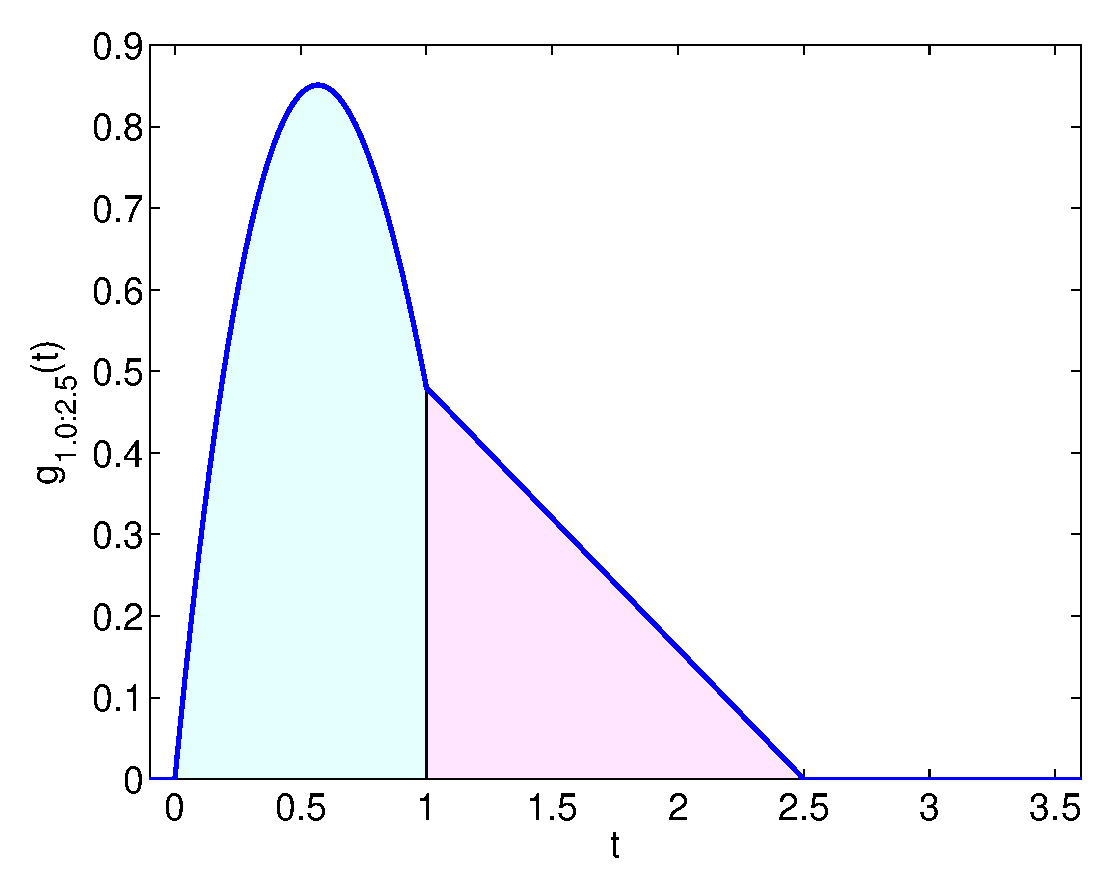
\includegraphics[width=0.48\columnwidth]{../Matlab/Plots/LinePicking_plot_rect_max_regions.eps}}
      \hspace{3mm}
    \subfloat[\label{fig:rect_max_pdf_var}PDF for various aspect
    ratios $a \! : \! b$ with $\max(a,b)=1$.]
        {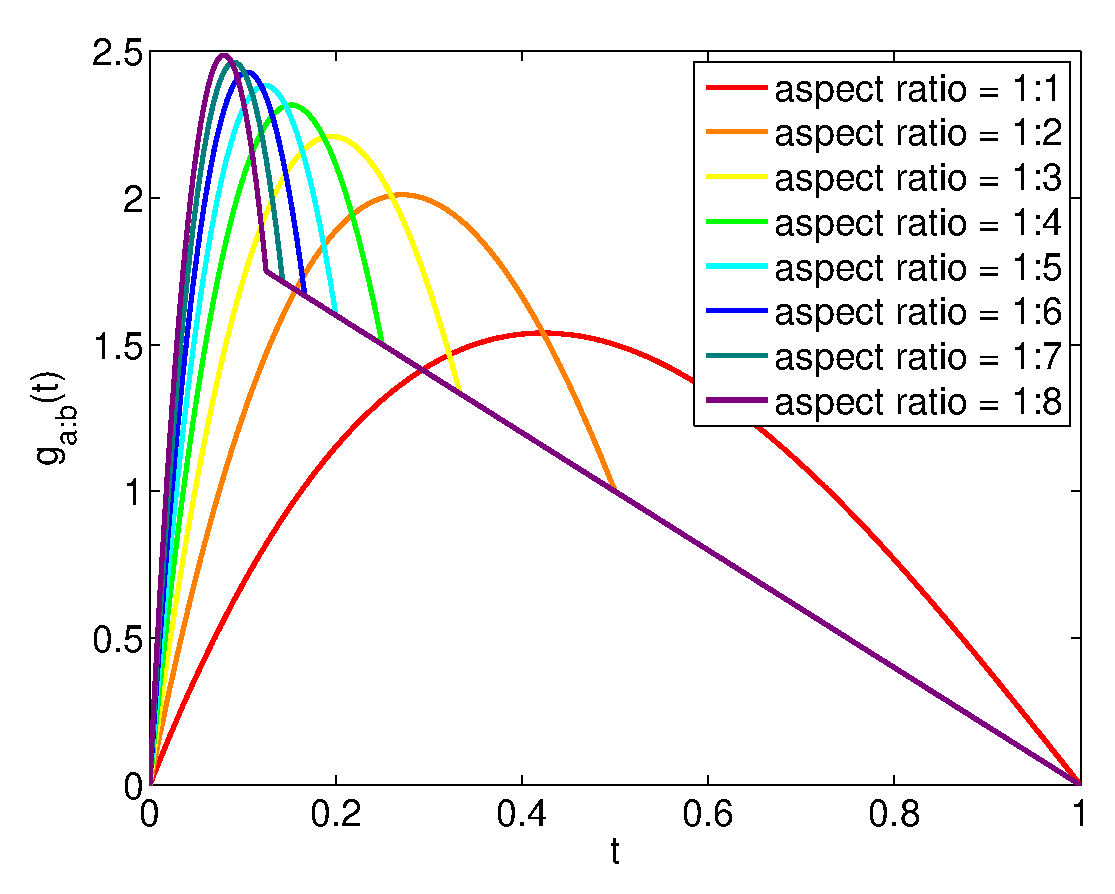
\includegraphics[width=0.48\columnwidth]{../Matlab/Plots/LinePicking_plot_rect_max.eps}}
    \caption{The line picking on the rectangle with the max metric.}
  \end{center} 
\vspace{-4mm}
\end{figure}  

\subsubsection{PDF}

Thus far all rectangular regions have resulted in a PDF made of three parts.
The elegant feature of this problem is that using the CDF method the rectangle 
can be partitioned into two parts. 

The  distance is the maximum of two independent random variables, i.e.,
\[ t_{\rm max} = \max (t_X,  t_Y), \]
where $t_X$ and $t_Y$ are distances given by the line-line picking
problem (Section~\ref{sec:line_line}). 

The probability density function of distances between two (uniformly) 
randomly chosen points on the unit line is given in
\eqref{eq:line_lineL}, and so the densities in the $X$ and $Y$
directions for a rectangle with sides $a$ and $b$ will be 
\begin{eqnarray}
  \label{eq:rect_xy}
  g^{\rm X}_b(t) & = & \left\{ \begin{array}{ll}
                    \frac{2}{b} \left( 1-\frac{t}{b} \right), &
                         \mbox{ for } 0 \leq t \leq b, \\
                    0, & \mbox{ otherwise}, \\
                  \end{array} \right. \nonumber \\
  g^{\rm Y}_a(t) & = & \left\{ \begin{array}{ll}
                    \frac{2}{a} \left( 1-\frac{t}{a} \right), &
                         \mbox{ for } 0 \leq t \leq a, \\
                    0, & \mbox{ otherwise}. \\
                  \end{array} \right. \nonumber 
\end{eqnarray}

Using the CDF method: 

\begin{equation}
 g^{\rm Max( X, Y)}_b(t) =
 \begin{cases}
 \frac {d  \int_{0}^{t} \int_{0}^{t}  g^{\rm X}_b g^{\rm Y}_a  dx\; dy }{dt} = \frac{2 t \left(4 a b-3 a t-3 b t+2 t^2\right)}{a^2 b^2} & 0 \le t < a \\ 
 \frac {d  \int_{0}^{a} \int_{a}^{t}  g^{\rm X}_b g^{\rm Y}_a  dx\; dy }{dt} = \frac{2 (b-t)}{b^2}& a \le t  \le b \\ 
 0 & \mbox{otherwise}
 \end{cases}
\end{equation}




\subsubsection{CDF}

The function above is comprised of two polynomial segments. A
closed form for the CDF is therefore easily derived:

\begin{equation}
 G^{\rm Max( X, Y)}_b(t) =
 \begin{cases}
 \frac{t^2 (2 a-t) (2 b-t)}{a^2 b^2} & 0 \le t < a \\ 
 \frac{t (2 b-t)}{b^2} & a \le t  \le b \\ 
 0 & t < 0\\
 1 & t > b
 \end{cases}
\end{equation}




\subsubsection{Moments}

Again because the PDF is made up of two polynomial segments calculating mean and variance is easy:

\begin{eqnarray}
 \mu &= &-\frac{a^3-5 a^2 b-10 b^3}{30 b^2}\\
 \sigma^{2} & = & -\frac{a^6-10 a^5 b+55 a^4 b^2-140 a^3 b^3+100 a^2 b^4-50 b^6}{900 b^4}
\end{eqnarray}








SHOULD DO A PLOT COMPARING THE 3 RECTANGLES WITH SAME SUPPORT







\clearpage
\subsection{Grid-line picking}
\label{sec:grid_line}

The grid-line picking problem takes points at random from a finite
grid, e.g., the integer points within a rectangle,
\[ \Z^{a,b} = \big\{ (x,y) \in \Z^2 \; \big| 
                      \; 0 \leq x \leq b \mbox{ and } 0 \leq y \leq a
              \big\},
\]
where $a, b \in \Z^+$.

Perhaps the most natural choice of metric here is the Manhattan
distance, but we could also approach the problem for the Euclidean
distance. 

\subsubsection{PDF}

This is an unusual case, in comparison to those above in that the
distribution is not continuous.

...

\subsubsection{CDF}

...


\subsubsection{Moments}

...





\clearpage
\subsection{Other examples involving rectangles}
\label{sec:rect_other}

In the problem formulation at the start of this paper we described the
line-picking problem as one where a line was chosen by choosing two
random points, independently, and drawing a ``line'' between them.  In
fact, some people interpret the idea of selecting a random line
differently.

Rosenberg~\cite{Rosenberg200499} considered the case where we first
choose a random angle, then choose the a random line within a
rectangle, such that it is at the required angle. 




 --- another way to think about it is choosing two points from a
 different space ....



\subsubsection{PDF}

???

\subsubsection{CDF}

???

\subsubsection{Moments}

Rosenberg~\cite{Rosenberg200499} derived the mean




\clearpage
\subsection{Cube-line picking}
\label{sec:cube_line}


\subsubsection{PDF}


\subsubsection{CDF}


\subsubsection{Moments}

\clearpage
\subsection{Hypercube max line picking}
\label{sec:hypercubemax_line}

The $n$-Dimensional hyper-cube (or just $n$-cube) with the {\em max} metric is particularly tractable.
Lower order examples are:
\begin{itemize}

\item A 1-cube is a line segment;

\item A 2-cube is a square;

\item A 3-cube is an ordinary cube.


\subsubsection{CDF}

We start by noting that the region is simply the cartesian product of $n$ lines and use the CDF method:

\begin{eqnarray}
 G^{n-{\rm cube max}}_L\left(t\right) & = & \int_{0}^{t} \ldots \int_{0}^{t}   g^{\rm line}_L\left(s_{1}\right)\ldots g^{\rm line}_L\left(s_{n}\right) \;ds_{1}\ldots ds_{n}, \nonumber \\
 & = & \int_{0}^{t}  g^{\rm line}_L\left(s_{1}\right) \;ds_{1}   \ldots \int_{0}^{t} g^{\rm line}_L\left(s_{n}\right) \;ds_{n},\nonumber \\
 & = & \left[\int_{0}^{t}  g^{\rm line}_L\left(s\right) \;ds \right]^{n},\nonumber \\
 & = & \left[G^{\rm line}_L\left(t\right)\right]^{n} ,\nonumber \\
 & = &  \left[\left(\frac{2}{L}\right)\left( t - \frac{t^2}{2L} \right)\right]^{n}.
\end{eqnarray}

\subsubsection{PDF}
To get the PDF we simply differentiate the PDF with respect to $t$:

\begin{eqnarray}
 g^{n-{\rm cube max}}_L\left(t\right) & = & \frac{d G^{n-{\rm cube max}}_L\left(t\right)}{dt},\nonumber \\
& = &  n\left[\left(\frac{2}{L}\right)\left( t - \frac{t^2}{2L} \right)\right]^{n-1} \left[\left(\frac{2}{L}\right)\left( 1 - \frac{t}{L} \right)\right],\nonumber \\
& = &  n\left(\frac{2}{L}\right)^{n} \left( t - \frac{t^2}{2L} \right)^{n-1}\left( 1 - \frac{t}{L} \right), \nonumber \\
\end{eqnarray} 
 
\subsubsection{Moments}

\begin{eqnarray}
E[ X^{k}_{n} ]  & = & \int_0^L t^k  g^{n-{\rm cube max}}_L\left(t\right) \, dt, \nonumber \\
& = &   n\left(\frac{2}{L}\right)^{n} \left(2L\right)^{k + n -1} \int_0^L \left(\frac{t}{2L}\right)^{k + n -1} \left( 1 - \frac{t}{2L} \right)^{n-1}\left( 1 - \frac{t}{L} \right) \; dt.
\end{eqnarray} 

Let $u = \frac{t}{2L}$ then $t = 2uL$ and $dt = du\; 2L$. Thus:
\begin{eqnarray}
E[ X^{k}_{n} ] & = &   n\left(\frac{2}{L}\right)^{n} \left(2L\right)^{k + n -1} \int_0^{\frac{1}{2}} u^{k + n -1} \left( 1 - u \right)^{n-1}\left( 1 - 2u} \right) \; du \; 2L, \nonumber \\
& = &   n 2^{2n + k} L^{k}\left[ \int_0^{\frac{1}{2}} u^{k + n -1} \left( 1 - u \right)^{n-1} \; du\  - 2\int_0^{\frac{1}{2}} u^{1+ k + n -1} \left( 1 - u \right)^{n-1} \; du\right], \nonumber \\
& = &   n 2^{2n + k} L^{k}\left[\beta\left(\frac{1}{2}; k + n, n\right) - 2\beta\left(\frac{1}{2}; k + n + 1, n\right)\right].  
\end{eqnarray}




\clearpage
\subsection{Hyperball-line picking}
\label{sec:hyperball_line}

The (closed) $n$-Dimensional hyperball (or just s$n$-ball) is the set
of points $B^n = \big\{ {\mathbf x} \in \R^n \; \big| \; \|{\mathbf x} \|_2 \leq R
\big\},$ where $R$ is the {\em radius}. For instance:
\begin{itemize}

\item A 1-ball is a line segment;

\item A 2-ball is a disk;

\item A 3-ball is an ordinary ball, i.e., the interior of a sphere.

\end{itemize}
In general, an $n$-ball is the interior of a $n-1$-sphere. 
% http://en.wikipedia.org/wiki/N-sphere

Figure~\ref{fig:hyperball_eg} shows an example of the line-picking
problem on the 2-ball (the disk). Generating points uniformly in an
$n-ball$ can be done by rejection (e.g., generating points uniformly
on an enclosing $n$-cube and sampling only those in the ball), or by
\begin{enumerate}

\item Choosing points uniformly on the surface. This can be
  accomplished by taking
  \begin{equation}
    \label{eq:x_surface_sphere}
    \x = R \frac{\y}{\| \y \|_2}, 
  \end{equation}
  where the $y_i \sim N(0,1)$ are IID standard normal random variates.

\item The find a point inside the $n$-ball by taking $u^{1/n} \x$,
  where $u \sim U([0,1])$ is uniformly generated from the interval $[0,1]$.

\end{enumerate}
The result is a set of points chosen so that the probability of there
being $k$ points inside non-overlapping regions of volume $v$ takes
IID Poisson distributions with mean $\lambda v$ where $\lambda =
m/V_n$, where $m$ is the total number of points generated, and $V_n$
is the volume of the $n$-ball.


\begin{figure}[tbp]
  \begin{center}
    \subfloat[\label{fig:hyperball_eg}2-ball
    example.]{\includegraphics[width=0.4\columnwidth]{../Matlab/Plots/LinePicking_test_sim_disk_eg.eps}} 
    \hspace{6mm}
    \subfloat[\label{fig:hyperball_pdf}PDF of $n$-balls.]{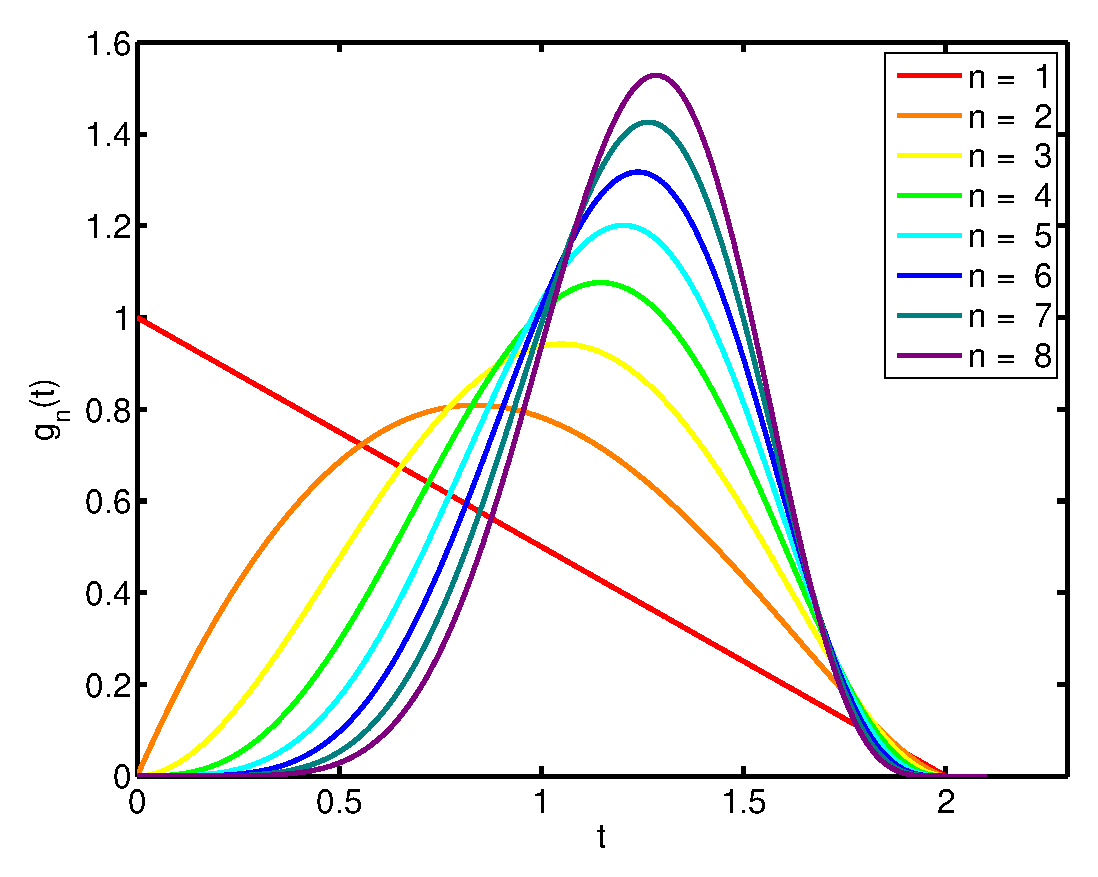
\includegraphics[width=0.48\columnwidth]{../Matlab/Plots/LinePicking_test_balls.eps}}
    \caption{The hyperball-line picking problem.}
  \end{center} 
\vspace{-4mm}
\end{figure}

\subsubsection{PDF}

Another obvious region on which to solve the line-picking problem is
the ball in $n$-dimensions~\cite{tu00:_circle_line} (equations
(27-31)). For a $n$-dimensional ball of radius $R$,
\begin{equation}
 g^{n-{\rm ball}}_R(t) = n \frac{t^{n-1}}{R^n} I_x\left( 
  \frac{1}{2} (n+1), \frac{1}{2}
                      \right),
\end{equation}
where
\begin{equation}
 x = 1 - \frac{t^2}{4 R^2}, 
\end{equation}
and $I_x(p,q)$ is a {\em regularized beta function}
\begin{equation}
   I_x(p,q) = \frac{ B(x; p,q)}{B(p,q)},
\end{equation}
where $B(x; p,q)$ is an incomplete beta function, and $B(p,q)$ is a
beta function, i.e., 
\begin{eqnarray}
  B(p,q)    & = & \int_0^1 t^{p-1} (1 - t)^{q-1} \, dt =
  \frac{\Gamma(p) \Gamma(q)}{\Gamma(p+q)}, \\
  B(x; p,q) & = & \int_0^x t^{p-1} (1 - t)^{q-1} \, dt.
\end{eqnarray}
The first few of these are \cite{tu00:_circle_line} ($P_2$ in (5) and
(17), $P_3$ in (9) and (19), $P_4$ in (18) and $P_5$ in (20), general
even form in (15), general odd form in (16)):
\begin{eqnarray}
  \label{eq:ball_line_picking}
  g^{1-{\rm ball}}_R(t) & = & \frac{1}{R} - \frac{t}{2 R}   \label{eq:line_line_picking}, \\
  g^{2-{\rm ball}}_R(t) & = & \frac{4 t}{\pi R^2} \cos^{-1} \left( \frac{t}{2R} \right)
               - \frac{2 t^2}{\pi R^3} \sqrt{1 - \frac{t^2}{4 R^2} } \label{eq:2dball_line_picking} , \\
          & = & \frac{2 t}{R^2} 
               - \frac{2 t^2}{\pi R^3} \sqrt{1 - \frac{t^2}{4 R^2} }
               - \frac{4 t}{\pi R^2} \sin^{-1} \left( \frac{t}{2R} \right) \label{eq:2dball_line_picking2} ,  \\
  g^{3-{\rm ball}}_R(t) & = & \frac{3 t^2}{R^3} - \frac{9 t^3}{4 R^4} + \frac{3 t^5}{16 R^6}   \label{eq:sphere_line_picking}  , \\
  g^{4-{\rm ball}}_R(t) & = &  \frac{8 t^3}{\pi R^4} \cos^{-1} \left( \frac{t}{2R} \right) 
              - \frac{8 t^4}{3 \pi R^5} \left( 1 - \frac{t^2}{4 R^2} \right)^{3/2}
               - \frac{4 t^4}{\pi R^5} \sqrt{1 - \frac{t^2}{4 R^2} } \\
  g^{5-{\rm ball}}_R(t) & = & \frac{5 t^4}{R^5} - \frac{75 t^6}{16 R^6} + \frac{25 t^7}{32 R^8} - \frac{15 t^9}{256 R^{10}} .
  \label{eq:ball_line_picking-end}
\end{eqnarray}
Tu and Fischbach \cite{tu00:_circle_line} also extend these results to
cases with non-uniform point distributions.
 
Figure~\ref{fig:hyperball_pdf} shows a comparison of line picking on
balls of various dimensions, and Figure~\ref{fig:various} shows a
comparison of the 2D and 3D balls to the square and cube. We can see
that as long as the areas (volumes) are matched, they appear quite
similar, respectively, though the rectangle varies considerably more.
% plot is similar to http://mathworld.wolfram.com/BallLinePicking.html

\subsubsection{CDF}

Take the case $R=1/2$ (we extend to the general case below), so that
\begin{equation}
 g^{n-{\rm ball}}_{1/2}(t) = n 2^n t^{n-1} I_{1-t^2}\left( 
  \frac{1}{2} (n+1), \frac{1}{2}
                      \right),
\end{equation}
where
\begin{equation}
   I_{1-t^2}(p,q) = 1 - I_{t^2}(q,p) = 1 - \frac{ B(t^2; q,p)}{B(q,p)}.
\end{equation}
So the CDF
\begin{eqnarray}
   G^{n-{\rm ball}}_{1/2}(\tau)
       & = & \int_0^\tau g^{n-{\rm ball}}_{1/2}(t) \, dt \nonumber \\
       & = &  \int_0^\tau n 2^n t^{n-1} \, dt 
            - \int_0^\tau n 2^n t^{n-1}  \frac{ B(t^2; q,p)}{B(q,p)} \, dt 
                  \nonumber \\
       & = &  2^n \tau^{n} 
            - \frac{n 2^n}{B(q,p)} \int_0^\tau t^{n-1}   B(t^2; q,p) \, dt .
\end{eqnarray}
Concentrating on the second term, and inserting the definition of the
incomplete $\beta$-function, we get 
\begin{eqnarray}
  n \int_0^\tau t^{n-1}  B(t^2; q,p) \, dt
       & = & n \int_{t=0}^\tau t^{n-1}  \int_{s=0}^{t^2} s^{q-1} (1 - s)^{p-1} \, ds \, dt \nonumber \\
       & = & n \int_{t=0}^\tau \int_{s=0}^{t^2} t^{n-1}  s^{q-1} (1 - s)^{p-1} \, ds \, dt \nonumber \\
       & = & n \int_{s=0}^{\tau^2} \int_{t=\sqrt{s}}^\tau t^{n-1}  s^{q-1} (1 - s)^{p-1} \, dt  \, ds \nonumber \\
       & = & n \int_{s=0}^{\tau^2}  s^{q-1} (1 - s)^{p-1} \int_{t=\sqrt{s}}^\tau t^{n-1} \, dt  \, ds \nonumber \\
       & = & \int_{s=0}^{\tau^2}  s^{q-1} (1 - s)^{p-1} \left[ t^{n} \right]_{t=\sqrt{s}}^\tau  \, ds \nonumber \\
       & = & \tau^n \int_{s=0}^{\tau^2}  s^{q-1} (1 - s)^{p-1} \, ds -
              \int_{s=0}^{\tau^2}  s^{n/2+q-1} (1 - s)^{p-1} \, ds \nonumber \\
       & = & \tau^n B(\tau^2; q,p) -  B(\tau^2; q+n/2,p).
\end{eqnarray}
Substituting back we get
\begin{eqnarray}
   G^{n-{\rm ball}}_{1/2}(\tau)
       & = &  2^n \tau^{n} 
            - \frac{n 2^n}{B(q,p)} \int_0^\tau t^{n-1}   B(t^2; q,p) \, dt  \nonumber \\
       & = &  2^n \left[ \tau^{n} \left(1-   \frac{B(\tau^2; q,p)}{B(q,p)} \right)
                           + \frac{B(\tau^2; q+n/2,p)}{B(q,p)} \right] \nonumber \\
       & = &  2^n \left[ \tau^{n} I_{1-\tau^2}(p,q)  + \frac{B(\tau^2; q+n/2,p)}{B(q,p)} \right],
\end{eqnarray}
where remember $p = \frac{1}{2} (n+1)$, and $q=\frac{1}{2}$.

Extending this to the general case with radius $R$ we get:
\begin{equation}
  \label{eq:cdf_n-ball}  
   G^{n-{\rm ball}}_{1/2}(\tau)
     =  2^n \left[ \left( \frac{\tau}{2R} \right)^{n} I_{x}(p,q)  + \frac{B(1-x; q+n/2,p)}{B(q,p)} \right].
\end{equation}

% also see http://mathworld.wolfram.com/IncompleteBetaFunction.html

\subsubsection{Moments}

Ghosh \cite{b.ghosh51:_random_rect} gives the first four moments of
the line-length distribution for the rectangle.
\begin{eqnarray}
  \label{eq:rect_moments} 
  \alpha_1 & = & \frac{1}{6} \left[ 
                        \frac{b^2}{a} \cosh^{-1}\left( M/b \right) +
                        \frac{a^2}{b} \cosh^{-1}\left( M/a \right) 
                 \right]
                  + \frac{1}{15} \left[ \frac{a^3}{b^2} + \frac{b^3}{a^2} \right]
                  - \frac{M}{15} \left[ \frac{a^2}{b^2} + \frac{b^2}{a^2} -3 \right],
\\
  \alpha_2 & = & \frac{1}{6} M^2, \\
  \alpha_3 & = & \frac{1}{20} \left[ 
                        \frac{b^4}{a} \cosh^{-1}\left( M/b \right) +
                        \frac{a^4}{b} \cosh^{-1}\left( M/a \right) 
                 \right]
                  + \frac{2}{105} \left[ \frac{a^5}{b^2} + \frac{b^5}{a^2} \right]
                  - \frac{2M}{105} \left[ \frac{a^4}{b^2} + \frac{b^4}{a^2}\right]
                        - \frac{5}{84} M^3, 
\\
  \alpha_4 & = & \frac{1}{15} a^4 + \frac{1}{18} a^2 b^2 + \frac{1}{15} b^4,
\end{eqnarray}
where $M = \sqrt{a^2 + b^2}$, from which we can derive the special
cases of the square and line (though these can also be derived
directly). Obvious central moments such as mean, and variance, etc.,
can be derived from these, though forumlas will be
complex. Rosenberg~\cite{Rosenberg200499} derives a similar result,
but under different assumptions of the random selection of lines (he
assumes we first choose a random angle, then choose the line.

The mean for the cube, known as the {\em Robbins constant}, is given
in \cite{robbins78:_constant,weisstein:_cube_line_picking} as
\begin{equation}
   \label{eq:cube_mean}
 \mu^{\rm cube} = \frac{1}{105} \left[ 
                             4 + 17 \sqrt{2}- 6 \sqrt{3}  +
                             21 \ln(1+\sqrt{2}) + 
                             42 \ln(2+\sqrt{3}) - 7 \pi
                      \right]
	=	0.66170...
\end{equation}
but a closed form for the variance does not appear (only even moments
are reported). Even more complicated results appear for 4- and 5-Cubes in
5-Cubes~\cite{philip:_probab_distr_distan_between_two_4d}:
\begin{eqnarray}
 \mu^{\rm 4-cube} & = & 0.7776656535 ...    \label{eq:4-cube}, \\
 \mu^{\rm 4-cube} & = & 0.8785309152 ...     \label{eq:5-cube}.
\end{eqnarray}

The means for the $n$-dimensional ball (with radius 1) are given in
\cite{weisstein:_ball_line_picking} as
\begin{eqnarray}
  \label{eq:ball-ndim-mean}
  \mu^{1D-{\rm ball}} & = & \frac{2}{3}, \\
  \mu^{2D-{\rm ball}} & = & \frac{128}{45 \pi},\\
  \mu^{3D-{\rm ball}} & = & \frac{36}{35}, \\
  \mu^{4D-{\rm ball}} & = & \frac{16384}{4725 \pi}.
\end{eqnarray}
The more general form for higher order moments is given in
\cite{tu00:_circle_line} (equation (138-141)) as
\begin{eqnarray}
  \label{eq:ball-ndim-moments}
  \alpha_m^{nD-{\rm ball}} & = &
     \frac{n 2^{m+n}}{m+n} \frac{B\left(\frac{n+1}{2}, \frac{n+m+1}{2}  \right)}{B\left(\frac{n+1}{2}, \frac{1}{2} \right)} R^m, \\
       & = & \left( \frac{n}{n+m} \right)^2 
                 \frac{\Gamma\left( n+m+1 \right) \Gamma\left( n/2 \right) }
                      {\Gamma\left( (n+m)/2 \right) \Gamma\left( n+1 + m/2 \right) } R^m.  
\end{eqnarray}
for and $n$-dimensional ball of radius $R$.









\clearpage
\subsection{$n$D-Sphere-line picking}
\label{sec:nsphere_line}

Can we do this case in general ???

$n$-Sphere is embedded in $\R^{n+1}$ and encloses the $n+1$-ball

\subsubsection{PDF}

Obviously, the sphere has spherical symmetry, but as a result, we can,
without loss of generality, assume the first point lies at the pole of
the sphere.

Points on the $n$-sphere can be parameterised by a set of angles
$\phi_1, \phi_2, \ldots, \phi_{n-1}$ where $\phi_1, \phi_2, \ldots,
\phi_{n-2}\in [0,\pi]$ and $\phi_{n-1}\in [0,2\pi)$. 


We can transform to Cartesian coordinates of $\R^{n+1}$ by
\begin{eqnarray}
  \label{eq:sphere_to_cart1}
  x_1 & = & R \cos (\phi_1 ) \\
  x_2 & = & R \sin(\phi_1) \cos (\phi_2 ) \\
  x_3 & = & R \sin(\phi_1) \sin(\phi_2) \cos (\phi_3 ) \\
      & \vdots & \\
  x_{n} & = & R \sin (\phi_1) \sin(\phi_2) \cdots \sin (\phi_{n-1}) \cos (\phi_{n})  \\
  x_{n+1} & = & R \sin (\phi_1) \sin(\phi_2) \cdots \sin (\phi_{n-1}) \sin (\phi_{n}) 
  \label{eq:sphere_to_cartn}
\end{eqnarray}

So the first point is chosen at the pole where
$\phi_1=\phi_2=\cdots=\phi_{n-1}=0$, so that ${\mathbf x} =
(R,0,0,\ldots,0)$, and the second point satisfies equations
\eqref{eq:sphere_to_cart1}-\eqref{eq:sphere_to_cartn}. 

Distance is therefore
\begin{eqnarray}
  \label{eq:d_nsphere}
  d^2 & = & R^2 \left[ 
                        (1-\cos(\phi_1))^2
                       + \sin^2 (\phi_1) \cos^2 (\phi_2 )
                       + \sin^2 (\phi_1) \sin^2 (\phi_2) \cos^2 (\phi_3 )
                       + \cdots \right.  \nonumber \\
     & &   \left.           + \sin^2 (\phi_1) \sin^2 (\phi_2) \cdots \sin^2 (\phi_{n-1}) \cos^2 (\phi_{n})
                       + \sin^2 (\phi_1) \sin^2 (\phi_2) \cdots \sin^2 (\phi_{n-1}) \sin^2 (\phi_{n}) 
                 \right].
\end{eqnarray}
The last two terms sum, using $\cos^2 (\phi_{n}) + \sin^2
(\phi_{n}) = 1$, and then the resulting last two terms sum
likewise, and so on collapsing the whole sum down to
\begin{eqnarray}
  \label{eq:d_nsphere}
  d^2 & = & R^2 \left[ 
                        (1-\cos(\phi_1))^2
                       + \sin^2 (\phi_1) \right], \nonumber \\
 & = & R^2 \left[ 1 - 2 \cos(\phi_1) + \cos^2(\phi_1)
                       + \sin^2 (\phi_1) \right], \nonumber \\
 & = & 2 R^2 \left[ 1 - \cos(\phi_1) \right].
\end{eqnarray}
So distance only depends on the first (angular) coordinate.


Uniformly chosen at random means that in any (generalized) area
element of size $d^{n}S$, there will be, on average $\lambda d^{n}S$
points (where $\lambda$ is the rate of points, which is simply the
total number of points divided by the total (generalized) area).

A small area unit on the $n$-sphere can be written (in terms of the
Jacobian $J$)
\begin{eqnarray}
  \label{eq:vn_n_sphere}
  d^nS & = & J \, d\phi_1 \, d\phi_2 \, \cdots d\phi_{n},  \nonumber \\
       & = & \sin^{n-1}(\phi_1) \sin^{n-2}(\phi_2) \cdots \sin(\phi_{n-1})
                  d\phi_1 \, d\phi_2 \, \cdots d\phi_{n}.
\end{eqnarray}
To obtain the distribution for distances, we integrate the distance
function over these elements to obtain the density of the first
angular coordinate, i.e.,
\begin{eqnarray}
  f(\phi_1)
      & = & \sin^{n-1}(\phi_1)
              \int_{0}^{2\pi} \int_{0}^{\pi} \cdots  \int_{0}^{\pi} 
              \sin^{n-2}(\phi_2) \cdots \sin(\phi_{n-1})
                   d\phi_2 \, \cdots d\phi_{n}, \nonumber \\
      & = & \sin^{n-1}(\phi_1)
              \int_{0}^{2\pi} 1 d\phi_{n} 
              \int_{0}^{\pi} \sin(\phi_{n-1}) d\phi_{n-1}  
              \cdots  
              \int_{0}^{\pi} \sin^{n-2}(\phi_2)  d\phi_{2}, \nonumber \\   
\end{eqnarray}
Now for $i>-1$, the integral % Wolfram alpha
\begin{equation}
  \label{eq:int_sin_n}
  \int_0^{\pi} \sin^i(x) \, dx = 
       \frac{\sqrt{\pi} \Gamma\big( i/2 + 1/2 \big)}{\Gamma\big( i/2+1 \big)}.
\end{equation}
Note that in each adjacent term in the product above, the Gamma
functions in the numerators and denominators cancel so the final
product collapses down to
\begin{eqnarray}
  f(\phi_1)
      & = & \sin^{n-1}(\phi_1)
              \int_{0}^{2\pi} 1 d\phi_{n} 
              \int_{0}^{\pi} \sin(\phi_{n-1}) d\phi_{n-1}  
              \cdots  
              \int_{0}^{\pi} \sin^{n-2}(\phi_2)  d\phi_{2}, \nonumber \\   
      & = & 2 \pi \pi^{(n-2)/2} \sin^{n-1}(\phi_1)  
                     \frac{\Gamma\big( 1/2 + 1/2 \big)}{\Gamma\big( (n-2)/2+1 \big)}
                 \nonumber \\   
      & = & 2 \pi^{n/2} \sin^{n-1}(\phi_1)  
                     \frac{\Gamma\big(1 \big)}{\Gamma\big( n/2 \big)}
                 \nonumber \\   
      & = &  2 \pi \sin^{n-1}(\phi_1)  
                     \frac{2 \pi^{(n-2)/2}}{\Gamma\big( (n-2)/2+1 \big)}
                 \nonumber \\   
      & = &   \frac{2 \pi \sin^{n-1}(\phi_1)}{C_{n-2}}
                 \nonumber \\   
\end{eqnarray}


The generalized volume and surface are of the $n$-D hyperball are
\begin{eqnarray}
 V_n(R) & = & C_n R^n,
  \label{eq:gen_vol} \\
 S_{n-1}(R) & = & \frac{dV_n}{dR} = n C_n R^{n-1}.
  \label{eq:gen_surf}
\end{eqnarray}
where
\begin{equation}
  \label{eq:cn}
   C_n = \frac{ \pi^{n/2} }{\Gamma(n/2 + 1)},
\end{equation}

where the Gamma function satisfies\cite[6.1.12]{Abramowitz_and_Stegun}
\begin{eqnarray}
  \label{eq:gamma}
  \Gamma(1/2) & = & \pi^{1/2}, \\
  \Gamma(3/2) & = & \frac{1}{2} \pi^{1/2}, \\
  \Gamma(k+1) & = & k!, \\
  \Gamma(k+1/2) & = & \frac{(2k)! \pi^{1/2}}{2^{2k} k!},
\end{eqnarray}
So we can write
\begin{eqnarray}
   \int_0^{\pi} \sin^i(x) \, dx
     & = & \left\{ \begin{array}{ll}
         \displaystyle
       \frac{\sqrt{\pi} \Gamma\big( n/2 + 1/2 \big)}{\Gamma\big( n/2+1 \big)}.
       & \mbox{ for } i = 2k, \\
         \displaystyle
       \frac{\sqrt{\pi} \Gamma\big( n/2 + 1/2 \big)}{\Gamma\big( n/2+1 \big)}.
       & \mbox{ for } i = 2k+1, \\
            \end{array} \right. \nonumber \\
\end{eqnarray}

We aim to have $f d\phi_1$ be uniform ????

So, say for $n=2$, we have
\begin{eqnarray}
  f(\phi_1)
      & = &   \frac{2 \pi \sin^{n-1}(\phi_1)}{C_{n-2}}
                 \nonumber \\   
      & = &   \frac{2 \pi \sin(\phi_1)}{C_{0}}
                 \nonumber \\   
      & = &   2 \pi \sin(\phi_1)  \nonumber \\   
  d^2 & = & 2 R^2 \left[ 1 - \cos(\phi_1) \right].  \nonumber \\  
\end{eqnarray}

Take 

\begin{eqnarray}
  \phi_1 & =  & \cos^{-1} \left[1-\frac{d^2}{2 R^2}\right]\\ 
   \frac {d \phi_1}{dd} & = &\frac{d}{\sqrt{1-\left(1-\frac{d^2}{2 R^2}\right)^2} R^2} \\
   & = &\frac{2}{\sqrt{4 R^2 -d^2 }}\\
\end{eqnarray}

thus 

\begin{equation}
  fd(d) & =  & \frac{2}{\sqrt{4 R^2 -d^2 }} fd_{\phi}(\frac{d}{\sqrt{1-\left(1-\frac{d^2}{2 R^2}\right)^2} R^2})
\end{equation}


\begin{eqnarray}
  prob(\phi_1) & = & 1/f(\phi_1) \nonumber \\  
      & = &  1/ 2 \pi \sin(\phi_1)
\end{eqnarray}


If $y = g(X)$

\[ f_Y(y) = \left| \frac{d}{dy} \left( g^{-1}(y) \right) \right|
                f_X\left( g^{-1}(y) \right)
\]


\begin{eqnarray}
  E[ g(X) ] & = & \int y f_g (y) \, dy \\
            & = & \int g(x) f_X(x) \, dx 
\end{eqnarray}


\subsubsection{CDF}


\subsubsection{Moments}


\clearpage
\subsection{$n$D-Sphere-geodesic-line picking}
\label{sec:nsphere_geodesic_line}

Sphere-geodesic-line picking is similar to sphere-line picking, except
that the ``lines'' are geodesics on the surface of the sphere, and the
distance metric is the length of these lines.

Can we do this case in general ??? Yes we can all the way down to the circle which gives a uniform distribution.

$n$-Sphere is embedded in $\R^{n+1}$ and encloses the $n+1$-ball


Figures ...

\begin{figure}[tbp]
  \begin{center}
    \subfloat[\label{fig:sphere_geo_eg}Example.]
       {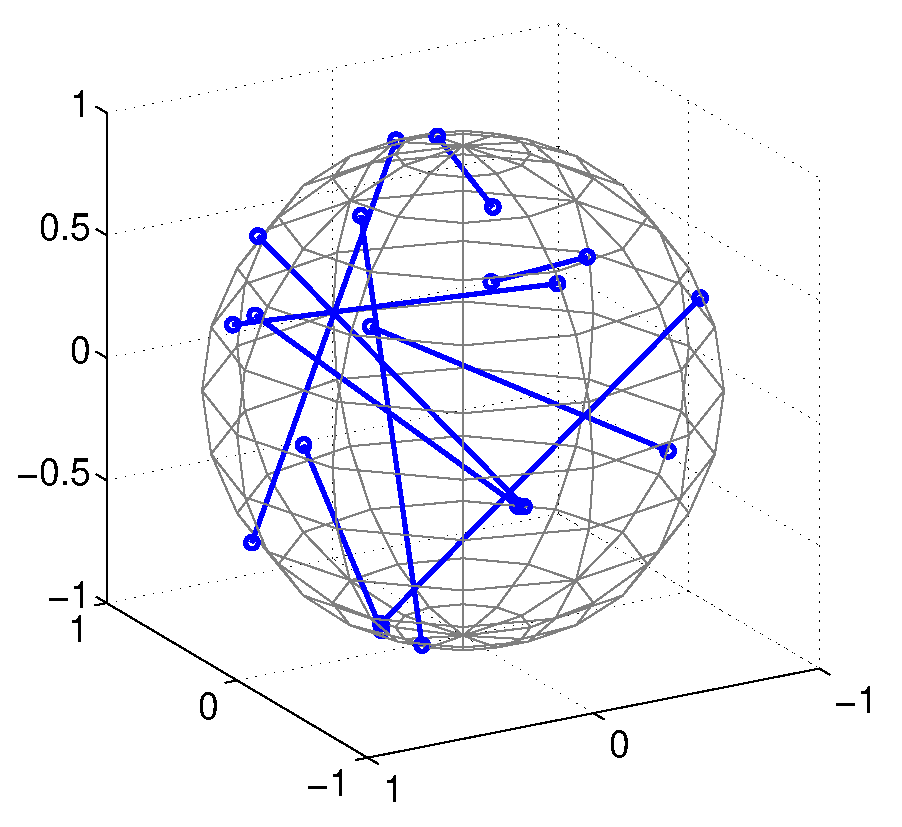
\includegraphics[width=0.4\columnwidth]{../Matlab/Plots/LinePicking_eg_sphere.eps}} 
    \hspace{6mm}
    \subfloat[\label{fig:sphere_geo_pdf}PDF.]
       {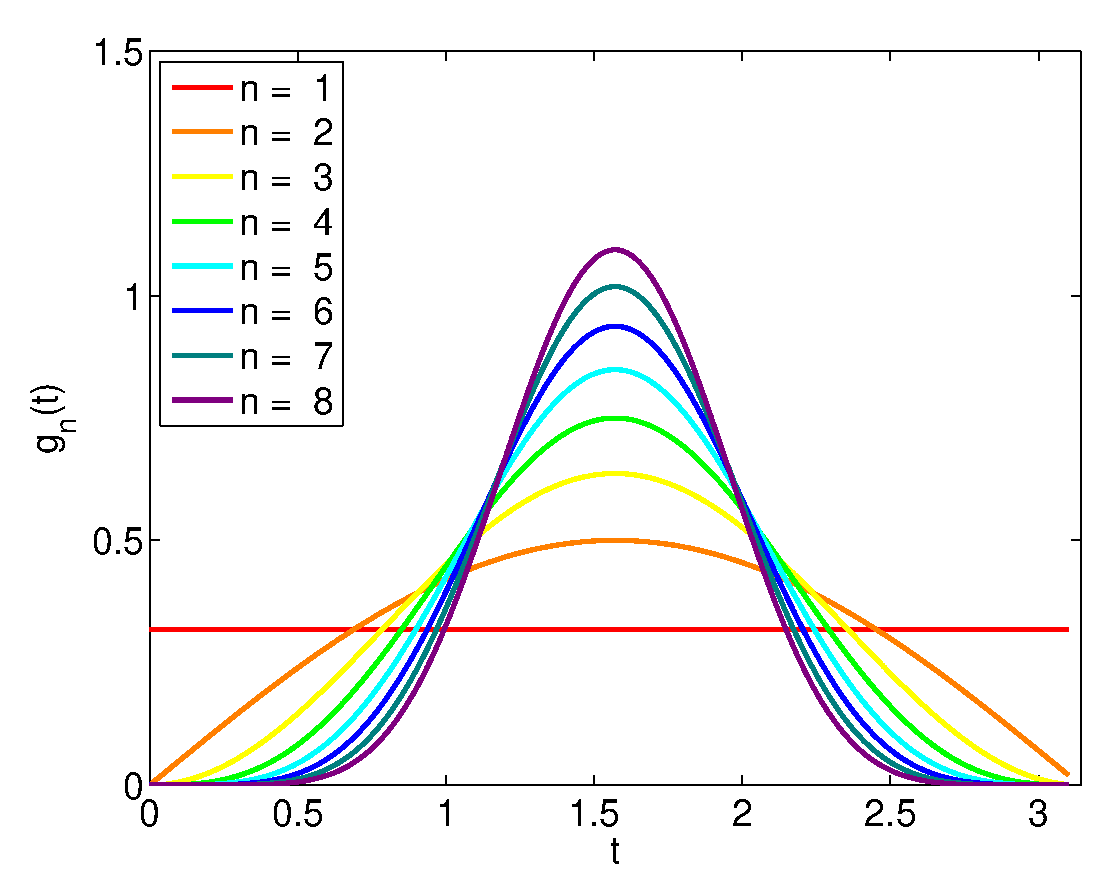
\includegraphics[width=0.48\columnwidth]{../Matlab/Plots/LinePicking_plot_nspheres_geodesic.eps}}
    \caption{The sphere-geodesic-line picking problem.}
  \end{center} 
\vspace{-4mm}
\end{figure}



\subsubsection{PDF}

Obviously, the sphere has spherical symmetry, but as a result, we can,
without loss of generality, assume the first point lies at the pole of
the sphere.

As in the $n$-Sphere above we first determine a density $f(\phi_1)$ function for $\phi_1$ then using the transform method. In fact $f(\phi_1)$ is exactly the same function as in the  $n$-Sphere thus we have:

\begin{equation}  
 f(\phi_1) = \frac{\Gamma\left(\frac{1+n}{2}\right) \sin(\phi )^{n - 1}}{\sqrt{\pi } \Gamma\left(\frac{n}{2}\right)}
\end{equation} 

We have have a function for $d$ the distance between two points in terms of $\phi_1$ so we can get  $\phi_1$ in terms of $d$ thus:

\begin{eqnarray}
  d & = & \phi_1  R.\\
\phi_1& = & \frac{d}{R}\\ 
   \frac {d \frac{d}{R}}{dd} & = & \frac{1}{R}\\
\end{eqnarray}



If $y = g(X)$ then the transform rule  is :  

\[ f_Y(y) = \left| \frac{d}{dy} \left( g^{-1}(y) \right) \right|
                f_X\left( g^{-1}(y) \right)
\]

thus 
\begin{eqnarray}
g_{R}^{n}(d) & = &  \left|\frac{1}{R}\right|  f\left(\frac{d}{R} \right)\\
 & = &\frac{\Gamma\left(\frac{1+n}{2}\right) \sin\left(\frac{d}{R}\right)^{n-1}}{\sqrt{\pi } R \Gamma\left(\frac{n}{2}\right)}
\end{eqnarray}

\subsubsection{CDF}
\begin{equation}
G_{R}^{n}(d)=\frac{1}{2}-\frac{\cos\left(\frac{d}{R}\right) \sin\left(\frac{d}{R}\right)^n \left(\sin\left(\frac{d}{R}\right)^2\right)^{-n/2}\Gamma\left(\frac{1+n}{2}\right) {}_{2}F_{1}\left(\frac{1}{2},1-\frac{n}{2},\frac{3}{2},\cos\left(\frac{d}{R}\right)^2\right) }  {\sqrt{\pi } \Gamma\left(\frac{n}{2}\right)}
\end{equation}

\subsubsection{Moments}

\begin{equation}
E[g_{R}^{n}(d)]=\frac{\pi R}{2}
\end{equation}






\clearpage
\subsection{Right Cylinder geodesic-line picking}
\label{sec:prism_geodesic_line}

Let the random variable $W$ describe the shortest distance (measured across the surface geodesically)between two points chosen randomly on the lateral surface of a right cylinder of length $L$ and perimeter $P$ with $L >P$ (note the bases of the cylinder need not be circles hence we derive in terms of the length of the perimeter of the base).  


Then $W$ has $p.d.f$
\begin{equation}
 \text{f}{w}(w) =
 \begin{cases}
  \frac{2 w (\pi  L-2 w)}{L^2 P} & 0 \le w < P \\
 \frac{4 w \arcsin\left(\frac{P}{2 w}\right)}{L P}-\frac{2 w}{L^2}& P\le w <  L \\
 \frac{4 w \sqrt{w^2-L^2}}{L^2 P}-\frac{2 w}{L^2}-\frac{4w \left( \arccos\left(\frac{L}{w}\right)- \arcsin\left(\frac{P}{2 w}\right)\right)}{L P} & L \le w < \sqrt{\left(\frac{P}{2}\right)^2+L^2}\\
 0 & \mbox{otherwise}
 \end{cases}
\end{equation}



\begin{align*}
I_{1}= & \intop_{0}^{w}\intop_{0}^{\sqrt{w^{2}-r^{2}}}\!\frac{4(1-\frac{d}{L})}{PL}\, dd\, dr,\\
= & \intop_{0}^{w}\!\left[\frac{4d}{PL}-\frac{2d^{2}}{PL^{2}}\right]_{0}^{\sqrt{w^{2}-r^{2}}}\, dr,\\
= & \intop_{0}^{w}\!\frac{4\sqrt{w^{2}-r^{2}}}{PL}-\frac{2(w^{2}-r^{2})}{PL^{2}}\, dr,\\
= & \frac{4}{PL}\intop_{0}^{w}\!\sqrt{w^{2}-r^{2}}\, dr+\frac{2}{PL^{2}}\intop_{0}^{w}\! r^{2}-w^{2}\, dr,\\
= & \frac{4w^{2}}{PL}\left[\frac{\arcsin(\frac{r}{w})}{2}+\frac{r\sqrt{1-(\frac{r}{w})^{2}}}{2w}\right]_{0}^{w}+\frac{2}{PL^{2}}\left[\frac{r^{3}}{3}-w^{2}r\right]_{0}^{w},\\
= & \frac{\pi w^{2}}{PL}-\frac{4w^{3}}{3PL^{2}}.\end{align*}


Now the second integral

\begin{align*}
I_{2}= & \intop_{0}^{\frac{P}{2}}\intop_{\sqrt{\left(\frac{P}{2}\right)^{2}-r^{2}}}^{\sqrt{w^{2}-r^{2}}}\!\frac{4(1-\frac{d}{L})}{PL}\, dd\, dr,\\
= & \intop_{0}^{\frac{P}{2}}\!\left[\frac{4d}{PL}-\frac{2d^{2}}{PL^{2}}\right]_{\sqrt{\left(\frac{P}{2}\right)^{2}-r^{2}}}^{\sqrt{w^{2}-r^{2}}}\, dr,\\
= & \intop_{0}^{\frac{P}{2}}\!\frac{4\sqrt{w^{2}-r^{2}}}{PL}-\frac{2\left(w^{2}-r^{2}\right)}{PL^{2}}-\frac{4\sqrt{\left(\frac{P}{2}\right)^{2}-r^{2}}}{PL}+\frac{2\left(\left(\frac{P}{2}\right)^{2}-r^{2}\right)}{PL^{2}}\, dr,\\
= & \frac{4}{PL}\intop_{0}^{\frac{P}{2}}\!\sqrt{w^{2}-r^{2}}\, dr-\frac{4}{PL}\intop_{0}^{\frac{P}{2}}\!\sqrt{\left(\frac{P}{2}\right)^{2}-r^{2}}\,\, dr+\frac{2}{PL^{2}}\intop_{0}^{\frac{P}{2}}\!\left(\frac{P}{2}\right)^{2}-w^{2}\, dr,\\
= & \frac{4}{PL}w^{2}\left[\frac{\arcsin\left(\frac{r}{w}\right)}{2}+\frac{r\sqrt{1-\left(\frac{r}{w}\right)^{2}}}{2w}\right]_{0}^{\frac{P}{2}}-\frac{P}{L}\left[\frac{\arcsin\left(\frac{2r}{P}\right)}{2}+\frac{r\sqrt{1-\left(\frac{2r}{P}\right)^{2}}}{P}\right]_{0}^{\frac{P}{2}}\\
& +\frac{2}{PL^{2}}\left[\left(\frac{P}{2}\right)^{2}r-w^{2}r\right]_{0}^{\frac{P}{2}},\\
= & \frac{2w^{2}\arcsin\left(\frac{P}{2w}\right)}{PL}+\frac{\sqrt{4w^{2}-P^{2}}}{2L}-\frac{\pi P}{4L}+\frac{\left(P^{2}-4w^{2}\right)}{4L^{2}}.\end{align*}


\begin{align*}
I_{3}= & \intop_{L}^{w}\intop_{0}^{\sqrt{w^{2}-d^{2}}}\!\frac{4(1-\frac{d}{L})}{PL}\, dr\, dd,\\
= & \intop_{L}^{w}\!\left[\frac{4r(L-d)}{PL^{2}}\right]_{0}^{\sqrt{w^{2}-d^{2}}}\, dd,\\
= & \frac{4}{PL}\intop_{L}^{w}\!\sqrt{w^{2}-d^{2}}\, dd-\frac{4}{PL^{2}}\intop_{L}^{w}\! d\sqrt{w^{2}-d^{2}}\, dd,\\
= & \frac{4w^{2}}{PL}\left[\frac{\arcsin\left(\frac{d}{w}\right)}{2}+\frac{d\sqrt{1-\left(\frac{d}{w}\right)^{2}}}{2w}\right]_{L}^{w}+\frac{4}{3PL^{2}}\left[(w^{2}-d^{2})\sqrt{w^{2}-d^{2}}\right]_{L}^{w},\\
= & \frac{\pi w^{2}}{PL}-\frac{2w^{2}\arcsin\left(\frac{L}{w}\right)}{PL}-\frac{2\sqrt{w^{2}-L^{2}}}{P}-\frac{4w^{2}\sqrt{w^{2}-L^{2}}}{3PL^{2}}+\frac{4\sqrt{w^{2}-L^{2}}}{3P},\\
\\= & \frac{2w^{2}\arccos\left(\frac{L}{w}\right)}{PL}-\frac{2\sqrt{w^{2}-L^{2}}}{3P}-\frac{4w^{2}\sqrt{w^{2}-L^{2}}}{3PL^{2}}.\end{align*}



\clearpage
\subsection{Right Cylinder line picking}
\label{sec:cylinder_line}

Let the random variable $W$ describe the shortest distance (measured across tbetween two points chosen randomly on the lateral surface of a right cylinder of length $L$ and diameter $D$ with $L >D$ 


\begin{align*}
f_{d}(d)=&\frac{2 \left(1-\frac{d}{L}\right)}{L}\\
f_{r}(r)=&\frac{2}{\pi  \sqrt{\text{D}^2-r^2}}\\
f_{r,d}(r,d)=&\frac{4 \left(1-\frac{d}{L}\right)}{\pi  L \sqrt{\text{D}^2-r^2}}
\end{align*}

\begin{align*}
I_{1}=&\intop_{0}^{w}
\intop_{0}^{\sqrt{w^{2}-r^{2}}}\!\!\!\!\!\!
\frac{4 \left(1-\frac{d}{L}\right)}{\pi  L \sqrt{\text{D}^2-r^2}}\,dd\,dr\\
%different factor
=&\intop_{0}^{w}
\intop_{0}^{\sqrt{w^{2}-r^{2}}}\!\!\!\!\!\!
\frac{4}{\pi  L \sqrt{\text{D}^2-r^2}} 
-\frac{4 d}{\pi  L^{2} \sqrt{\text{D}^2-r^2}}
\,dd\,dr\\
%integrate inner 
=&\intop_{0}^{w}
\left[
\frac{4 d}{\pi  L \sqrt{\text{D}^2-r^2}} 
-\frac{2 d^{2}}{\pi  L^{2} \sqrt{\text{D}^2-r^2}}
\right]_{0}^{\sqrt{w^{2}-r^{2}}}
\,dr\\
% substitute in upper and lower limits
=&
\intop_{0}^{w}\!
\frac{4 \sqrt{w^2-r^2}}{\pi  L\sqrt{\text{D}^2-r^2}}
-\frac{2 w^2}{\pi  L^2 \sqrt{\text{D}^2-r^2}}
+\frac{2 r^2}{\pi  L^2\sqrt{\text{D}^2-r^2}}
\,dr\\
%break into integrals we know how to deal with
=&
\frac{4}{\pi  L}\!\!
\intop_{0}^{w}\!
\frac{\sqrt{w^2-r^2}}{\sqrt{\text{D}^2-r^2}}
\,dr
-\frac{2 w^2}{\pi  L^2 }\!\!
\intop_{0}^{w}\!
\frac{1}{\sqrt{\text{D}^2-r^2}}
\,dr
+\frac{2}{\pi  L^2}\!\!
\intop_{0}^{w}\!
\frac{r^2}{\sqrt{\text{D}^2-r^2}}
\,dr\\
%Further manipilation to get that first integral in the form of an elliptic integral
=&
\frac{4 w}{\pi  L \text{D}}\!\!
\intop_{0}^{w}\!
\frac{\sqrt{1-\left(\frac{r}{w}\right)^2}}{\sqrt{1-\left(\frac{r}{\text{D}}\right)^2}}
% second integral use http://www.integral-table.com/ equation 33
-\frac{2 w^2}{\pi  L^2 }\left[
\arcsin\left(\frac{r}{\text{D}}\right)
\right]_{0}^{w}
% third integral use http://www.integral-table.com/ equation 37 and use arctan(x) = arcsin(XXXXX) identity  from http://en.wikipedia.org/wiki/
+\frac{1}{\pi  L^2}\left[
\text{D}^{2}\arcsin\left(\frac{r}{\text{D}}\right)
-r\sqrt{\text{D}^2-r^2}
\right]_{0}^{w}\!\\
\end{align*}

For the first integrand let $s=\frac{r}{\text{D}}$ so $ds=\frac{1}{\text{D}}\,dr$ thus 

% get the first integral in the form of an elliptic integral of the second kind
\begin{align*}
I_{1}=&
\frac{4 w}{\pi  L }\!\!
\intop_{0}^{\frac{w}{\text{D}}}\!
\frac{\sqrt{1-\left(\frac{\text{D}}{w}\right)^{2}s^{2}}}{\sqrt{1-s^2}}
\,ds
% now substitute in the upper and lower bounds in the remaining integrals
-\frac{2 w^2}{\pi  L^2 }
\arcsin\left(\frac{w}{\text{D}}\right)
+\frac{\text{D}^{2}}{\pi  L^2 }\arcsin\left(\frac{w}{\text{D}}\right)
-\frac{w}{\pi  L^2}\sqrt{\text{D}^2-w^2}\\
% first integral is in the form of an elliptic integral of the second kind see  http://mathworld.wolfram.com/EllipticIntegraloftheSecondKind.html
=&\frac{4 w}{\pi  L }E\left(\arcsin\left(\frac{w}{\text{D}}\right),\frac{\text{D}^{2}}{w^{2}}\right)
+\frac{\text{D}^{2}-2 w^2}{\pi  L^2 }\arcsin\left(\frac{w}{\text{D}}\right)
-\frac{w}{\pi  L^2}\sqrt{\text{D}^2-w^2}\\
% now using the identity at http://functions.wolfram.com/EllipticIntegrals/EllipticE2/03/01/02/0004/ we get the incomplete elliptic integral of the second type in terms of complete elliptic integrals of the first and second type
=&\frac{4 \text{D}}{\pi  L }
\left(E\left(\frac{w^2}{\text{D}^2}\right)+\left(\frac{w^2}{\text{D}^2}-1\right)K\left(\frac{\text{D}^2}{w^2}\right)\right)
% second and third term combined
+\frac{\text{D}^{2}-2 w^2}{\pi  L^2 }\arcsin\left(\frac{w}{\text{D}}\right)
-\frac{w}{\pi  L^2}\sqrt{\text{D}^2-w^2}\\
\end{align*}

Now we do the second integral

\begin{align*}
I_{2}=&\intop_{0}^{\text{D}}
\intop_{\sqrt{\text{D}^{2}-r^{2}}}^{\sqrt{w^{2}-r^{2}}}\!\!\!
\frac{4 \left(1-\frac{d}{L}\right)}{\pi  L \sqrt{\text{D}^2-r^2}}\,dd\,dr\\
%different factor
=&\intop_{0}^{\text{D}}
\intop_{\sqrt{\text{D}^{2}-r^{2}}}^{\sqrt{w^{2}-r^{2}}}\!\!\!
\frac{4}{\pi  L \sqrt{\text{D}^2-r^2}} 
-\frac{4 d}{\pi  L^{2} \sqrt{\text{D}^2-r^2}}
\,dd\,dr\\
%integrate inner 
=&\intop_{0}^{\text{D}}
\left[
\frac{4 d}{\pi  L \sqrt{\text{D}^2-r^2}} 
-\frac{2 d^{2}}{\pi  L^{2} \sqrt{\text{D}^2-r^2}}
\right]_{\sqrt{\text{D}^{2}-r^{2}}}^{\sqrt{w^{2}-r^{2}}}
\,dr\\
% substitute in lower and upper limits and do a pile of simplification
=&
\intop_{0}^{\text{D}}\!
\frac{4 \sqrt{w^2-r^2}}{\pi  L\sqrt{\text{D}^2-r^2}}
+\frac{2 \left(\text{D}^2-w^2\right)}{\pi  L^2\sqrt{\text{D}^2-r^2}}
-\frac{4}{\pi  L}
\,dr\\
% split it up into parts suitable for using integrals from tables on
=&
\frac{4}{\pi  L}
\intop_{0}^{\text{D}}\!
\frac{\sqrt{w^2-r^2}}{\sqrt{\text{D}^2-r^2}}
\,dr
+\frac{2 \left(\text{D}^2-w^2\right)}{\pi  L^2}\!\!
\intop_{0}^{\text{D}}\!
\frac{1}{\sqrt{\text{D}^2-r^2}}
\,dr
-\frac{4}{\pi  L}
\intop_{0}^{\text{D}}\!
1
\,dr\\
%Further manipilation to get that first integral in the form of an elliptic integral
=&
\frac{4 w}{\pi  L \text{D}}\!\!
\intop_{0}^{\text{D}}\!
\frac{\sqrt{1-\left(\frac{r}{w}\right)^2}}{\sqrt{1-\left(\frac{r}{\text{D}}\right)^2}}
\,dr
% second integral use http://www.integral-table.com/ equation 33
+\frac{2 \left(\text{D}^2-w^2\right)}{\pi  L^2}\left[
\arcsin\left(\frac{r}{\text{D}}\right)
\right]_{0}^{\text{D}}
% third integral no tables required
-\frac{4}{\pi  L}\left[
r
\right]_{0}^{\text{D}}
\end{align*}

For the first integrand let $s=\frac{r}{\text{D}}$ so $ds=\frac{1}{\text{D}}\,dr$ thus
% get the first integral in the form of an elliptic integral of the second kind
\begin{align*}
I_{2}=&
\frac{4 w}{\pi  L }\!\!
\intop_{0}^{1}\!
\frac{\sqrt{1-\left(\frac{\text{D}}{w}\right)^{2}s^{2}}}{\sqrt{1-s^2}}
\,ds
+\frac{\left(\text{D}^2-w^2\right)}{ L^2}
-\frac{4 \text{D}}{\pi  L}\\
=&\frac{4 w}{\pi  L }E\left(\frac{\text{D}^2}{w^2}\right)
+\frac{\left(\text{D}^2-w^2\right)}{ L^2}
-\frac{4 \text{D}}{\pi  L}
\end{align*}

And the third integral

\begin{align*}
I_{3}=&\intop_{0}^{\sqrt{w^2-L^2}}
\intop_{L}^{\sqrt{w^{2}-r^{2}}}\!\!\!
\frac{4 \left(1-\frac{d}{L}\right)}{\pi  L \sqrt{\text{D}^2-r^2}}\,dd\,dr\\
%different factor
=&\intop_{0}^{\sqrt{w^2-L^2}}
\intop_{L}^{\sqrt{w^{2}-r^{2}}}\!\!\!
\frac{4}{\pi  L \sqrt{\text{D}^2-r^2}} 
-\frac{4 d}{\pi  L^{2} \sqrt{\text{D}^2-r^2}}
\,dd\,dr\\
%integrate inner 
=&\intop_{0}^{\sqrt{w^2-L^2}}
\left[
\frac{4 d}{\pi  L \sqrt{\text{D}^2-r^2}} 
-\frac{2 d^{2}}{\pi  L^{2} \sqrt{\text{D}^2-r^2}}
\right]_{L}^{\sqrt{w^{2}-r^{2}}}
\,dr\\
% substitute in lower and upper limits and do a pile of simplification 
=&\intop_{0}^{\sqrt{w^2-L^2}}\!
\frac{4 \sqrt{w^2-r^2}}{\pi  L\sqrt{\text{D}^2-r^2}}
-\frac{2 w^2}{\pi  L^2\sqrt{\text{D}^2-r^2}}
+\frac{2 r^2}{\pi  L^2\sqrt{\text{D}^2-r^2}}
-\frac{2}{\pi  \sqrt{\text{D}^2-r^2}}
\,dr\\
% split it up into parts suitable for using integrals from tables on
=&
\frac{4}{\pi  L}\!\!\!
\intop_{0}^{\sqrt{w^2-L^2}}\!\!\!
\frac{\sqrt{w^2-r^2}}{\sqrt{\text{D}^2-r^2}}
\,dr
-\frac{2 w^2}{\pi  L^2}\!\!
\intop_{0}^{\sqrt{w^2-L^2}}\!\!\!\!\!
\frac{1}{\sqrt{\text{D}^2-r^2}}
\,dr
+\frac{2}{\pi  L^2}\!\!
\intop_{0}^{\sqrt{w^2-L^2}}\!\!\!\!\!
\frac{r^2}{\sqrt{\text{D}^2-r^2}}
\,dr
-\frac{2}{\pi}
\intop_{0}^{\sqrt{w^2-L^2}}\!\!\!\!\!
\frac{1}{\sqrt{\text{D}^2-r^2}}
\,dr\\
%Further manipilation to get that first integral in the form of an elliptic integral
=&
\frac{4 w}{\pi  L \text{D}}\!\!
\intop_{0}^{\sqrt{w^2-L^2}}\!\!\!\!\!
\frac{\sqrt{1-\left(\frac{r}{w}\right)^2}}{\sqrt{1-\left(\frac{r}{\text{D}}\right)^2}}
\,dr
% second integral use http://www.integral-table.com/ equation 33
-\frac{2 w^2}{\pi  L^2}\left[
\arcsin\left(\frac{r}{\text{D}}\right)
\right]_{0}^{\sqrt{w^2-L^2}}\\
% third integral use http://www.integral-table.com/ equation 37 and use arctan(x) = arcsin(XXXXX) identity  from http://en.wikipedia.org/wiki/
&+\frac{1}{\pi  L^2}\left[
\text{D}^{2}\arcsin\left(\frac{r}{\text{D}}\right)
-r\sqrt{\text{D}^2-r^2}
\right]_{0}^{\sqrt{w^2-L^2}}
% fourth integral use http://www.integral-table.com/ equation 33
-\frac{2}{\pi}\left[
\arcsin\left(\frac{r}{\text{D}}\right)
\right]_{0}^{\sqrt{w^2-L^2}}
\end{align*}
\\
For the first integrand let $s=\frac{r}{\text{D}}$ so $ds=\frac{1}{\text{D}}\,dr$ thus

\begin{align*}
%Further manipilation to get that first integral in the form of an elliptic integral
I_{3}=&
\frac{4 w}{\pi  L }\!\!
\intop_{0}^{\frac{\sqrt{w^2-L^2}}{\text{D}}}
\!
\frac{\sqrt{1-\left(\frac{\text{D}}{w}\right)^{2}s^{2}}}{\sqrt{1-s^2}}
\,ds
% second integral use http://www.integral-table.com/ equation 33
+\frac{\text{D}^{2}-2 w^2-2L^2}{\pi  L^2}\left[
\arcsin\left(\frac{r}{\text{D}}\right)
\right]_{0}^{\sqrt{w^2-L^2}}
% third integral 
-\frac{1}{\pi  L^2}\left[
r\sqrt{\text{D}^2-r^2}
\right]_{0}^{\sqrt{w^2-L^2}}\\
%Write the elliptical integral as E
=&\frac{4 w}{\pi  L }E\left(\arcsin\left(\frac{\sqrt{w^2-L^2}}{\text{D}}\right),\frac{\text{D}^{2}}{w^{2}}\right)
+\frac{\text{D}^{2}-2 w^2-2L^2}{\pi  L^2 }\arcsin\left(\frac{\sqrt{w^2-L^2}}{\text{D}}\right)\\
&-\frac{\sqrt{\left(w^2-L^2\right) \left(\text{D}^2+L^2-w^2\right)}}{\pi  L^2}
\\
=&-\frac{4 w \sqrt{-\left(L^2-w^2\right) \left(D^2+L^2-w^2\right)}}{\pi 
   D^2 L^2}-\frac{4 \left(3 D^4 w \sec
   ^{-1}\left(\frac{D}{\sqrt{w^2-L^2}}\right)+16 D^2 L w^2
   K\left(\frac{D^2}{w^2}\right)-16 L w^4
   K\left(\frac{D^2}{w^2}\right)-12 D^2 L^2 w \sec
   ^{-1}\left(\frac{D}{\sqrt{w^2-L^2}}\right)-16 D^2 L w^2 F\left(\csc
   ^{-1}\left(\frac{D}{\sqrt{w^2-L^2}}\right)|\frac{D^2}{w^2}\right)-16
   D^2 L w^2 E\left(\csc
   ^{-1}\left(\frac{D}{\sqrt{w^2-L^2}}\right)|\frac{D^2}{w^2}\right)+16
   L w^4 F\left(\csc
   ^{-1}\left(\frac{D}{\sqrt{w^2-L^2}}\right)|\frac{D^2}{w^2}\right)-16
   L w^4 E\left(\csc
   ^{-1}\left(\frac{D}{\sqrt{w^2-L^2}}\right)|\frac{D^2}{w^2}\right)-12
   D^2 w^3 \sec ^{-1}\left(\frac{D}{\sqrt{w^2-L^2}}\right)+16
   D^2 L w^2 E\left(\frac{D^2}{w^2}\right)+16 L w^4
   E\left(\frac{D^2}{w^2}\right)\right)}{3 \pi  D^4 L^2}-\frac{8 w
   \sqrt{-\left(L^2-w^2\right) \left(D^2+L^2-w^2\right)}}{3 \pi 
   D^4}-\frac{8 w^3 \sqrt{-\left(L^2-w^2\right)
   \left(D^2+L^2-w^2\right)}}{\pi  D^4 L^2}
\end{align*}


\clearpage
\subsection{Nonuniform line picking example}
\label{sec:nonuniform_line}

An example of a non-uniform case, perhaps Gaussian distribution on nD
with infinite region?

Just to illustrate the concept


\subsubsection{PDF}


...

\subsubsection{CDF}

...


\subsubsection{Moments}

...





\clearpage
\subsection{Others}

Cylinder

Cylinder geodesic

Cube-face-to-face

Rectangle to Rectangle

Helix -- geodesic is obvious but Euclidean could be interesting, and
maybe a relevance to DNA
 

Lp norm -- e.g., generalize rectangle (sphere might be hard because
$cos^p+sin^p=1$ only works for p=2?)



\clearpage
\subsection{Summary}
SUMMARY TABLE -- at least giving equation and page references.

\begin{table}[ht]
  \centering
  \begin{tabular}{r|lllllllllll}
    Problem & Parameters & Mean & Variance & PDF & CDF \\
    \hline
    AUTOGENERATE
  \end{tabular}
  \caption{Summary of the examples considered here.}
  \label{tab:summary}
\end{table}

\clearpage



\section{Approximations}

For some problems, it may be interesting to understand the behaviour
of these distributions for small $t$. 

\subsection{Examples}

\subsubsection{Line}
For the line \eqref{eq:line_line} we need no approximation:
\begin{equation}
  g^{\rm line}_L(t) = \frac{2}{L} - \frac{2}{L^2} t.
\end{equation}

\subsubsection{Rectangle (and square)}
For the rectangle (and square) we need only restrict our attention to
the case $t<a$ (the smaller side length), to get a simple polynomial
expression: 
\begin{eqnarray}
  g^{\rm rect}_{a,b}(t) & = & 
           \frac{4 t}{a^2 b^2}  
         \left[ \frac{ab \pi}{2} - (a+b) t + \frac{t^2}{2} \right],
          \nonumber \\
                         & = & \frac{2 \pi}{A} t 
                              - \frac{2 P}{A^2} t^2
                              + \frac{2}{A^2} t^3,
\end{eqnarray}
where $A = ab$ is the area of the rectangle, and $P = a+b$ is the perimeter.

The affect of changing the scale must be obvious, in that we know area
scales quadratically, and perimeter linearly with the size of the
region, so simple dimensional analysis suggests a form such as that
above must occur, but it is perhaps suprising that it is so clean. 

\subsubsection{Cube (and box)}
For the cube~\cite{weisstein:_cube_line_picking}, for small $t$,
\begin{eqnarray}
  g^{\rm cube}_{1}(t) & = &  -t^2 \left[ (t-8)t^2 + \pi (6 t - 4) \right], \nonumber \\
                    & = & 4 \pi t^2 - 6 \pi t^3 + 8 t^4 - t^5.
\end{eqnarray}
For the box~\cite{philip:_probab_distr_distan_between_two} with $t < a
\leq b \leq c$, we first see the distribution  of $u=t^2$ (using $g(t)
= 2 t h(t^2)$, 
\begin{eqnarray}
  h^{\rm box}_{a,b,c}(u) & = &
  \frac{1}{6 a^2 b^2 c^2} \left[
    - 6 \pi b c u + 8 b u^{3/2}
    +12 \pi a b c \sqrt u - 6 \pi a(b + c)u + 8(a + c) u^{3/2} - 3 u^2
    \right], \nonumber \\
  g^{\rm box}_{a,b,c}(t)  & = &
  \frac{t }{3 a^2 b^2 c^2} \left[
    - 6 \pi b c t^2 + 8 b t^{3}
    +12 \pi a b c t - 6 \pi a(b + c)t^2 + 8(a + c) t^{3} - 3 t^4
    \right], \nonumber \\
 & = & \frac{4 \pi}{V} t^2
       + \frac{\pi }{3 V^2} \left[ -6 b c - 6 a (b+c) \right] t^3
       + \frac{1}{3 V^2} \left[ 8 b + 8 (a+c) \right] t^4
       + \frac{1}{3 V^2} \left[ - 3 \right] t^5, \nonumber \\
 & = & \frac{4 \pi}{V} t^2
       - \frac{2 \pi }{ V^2} \left[ a b + bc + a c \right] t^3
       + \frac{8}{3 V^2} \left[ a + b + c \right] t^4
       - \frac{1}{V^2} t^5,  \nonumber \\
 & = & \frac{4 \pi}{V} t^2
       - \frac{\pi S}{ V^2} t^3
       + \frac{2 P}{3 V^2}  t^4
       - \frac{1}{V^2} t^5, 
\end{eqnarray}
for volume $V = a b c$, surface area $S = 2(a b + bc + a c)$ and edge
perimeter $P = 4(a + b + c)$>


\subsubsection{Hyperball}

For the $n$-dimensional hyperball, simple approximations are available
by use of Taylor series. Ignoring the 1D case (which is the same as
the line), we see the 2D disk
from~\cite{tu00:_circle_line,weisstein:_circle_line_picking}: 
\[
   g^{2D-{\rm ball}}_R(t) 
     =  \frac{4 t}{\pi R^2} \cos^{-1} \left( \frac{t}{2R} \right) 
               - \frac{2 t^2}{\pi R^3} \sqrt{1 - \frac{t^2}{4 R^2} }          
\]
and we use
\begin{eqnarray*}
  \cos^{-1}(x)  & = & \frac{1}{2} \pi - x - \frac{1}{6} x^{3} + \cdots \\
  \sqrt{1 - x^2} & = & 1 - \frac{x^2}{2} - \frac{x^4}{8}  + \cdots.
\end{eqnarray*}
% http://www.wolframalpha.com/input/?i=Taylor+series+of+%288%2F%28pi*R%29%29*%28x*arccos%28x%29+-+x^2*sqrt%281-x^2%29+%29
% http://www.wolframalpha.com/input/?i=Taylor+series+of+%288%2F%28pi*R%29%29*%28%28t%2F%282*R%29*arccos%28t%2F%282*R%29%29+-+%28t%2F%282*R%29%29^2*sqrt%281-%28t%2F%282*R%29%29^2%29+%29
to derive
\begin{eqnarray}
  g^{2D-{\rm ball}}_R(t) 
         & = & \frac{4 t}{\pi R^2} \cos^{-1} \left( \frac{t}{2R} \right) 
               - \frac{2 t^2}{\pi R^3} \sqrt{1 - \frac{t^2}{4 R^2} }
               \nonumber \\
         & = & \frac{4 t}{\pi R^2} \left( \frac{1}{2} \pi - \frac{t}{2R} \right)
                   -  \frac{2 t^2}{\pi R^3} + O(t^4)  \nonumber \\
         & = &  \frac{2 t}{R^2} -  \frac{4 t^2}{\pi R^3}  + O(t^4) \nonumber \\
         & = &  \frac{2 \pi}{A} t -  \frac{2 P}{A^2} t^2 + O(t^4) 
\end{eqnarray}
where once again $A=\pi R^2$ and $P = 2 \pi R$ are area and perimeter,
respectively. We note that this is very similar to the formula
obtained for the square for small $t$. The first two terms are, in
fact, identical.

For the 3D ball we already have the expression as a polynomial:
\begin{eqnarray}
  g^{3D-{\rm ball}}_R(t) 
        & = & \frac{3 t^2}{R^3} - \frac{9 t^3}{4 R^4} + \frac{3 t^5}{16 R^6}  \nonumber , \\
        & = & \frac{4 \pi}{V} t^2 - \frac{\pi S}{V^2} t^3 + \frac{3}{16 R^6} t^5,
\end{eqnarray}
where again $V=4 \pi R^3/3$ and $S = 4 \pi R^2$ are the volume and
surface area. Interestingly, these are identical to those terms for
the cube, and even the forth order term is the same if we say that the
sphere has zero edges.


%%%%%%%%%%%%%%%%%%%%%%%%%%%%%%%%%%%%%%%%%%%%%%%%%%%%%%%%%%%%%%%%%%5


The more general expression for the $n$-D ball can be derived by
noting that for a $n$-dimensional ball of radius $R$,
\begin{equation}
 g^{nD-{\rm ball}}_R(t) = n \frac{t^{n-1}}{R^n} I_x\left( 
  \frac{1}{2} (n+1), \frac{1}{2}
                      \right),
\end{equation}
rememeber $x = 1 - t^2/4R^2$, $a=(n+1)/2$, and $b=1/2$, and from
\cite[26.5.4]{Abramowitz_and_Stegun}
\begin{eqnarray}
  \label{eq:Ix}
  I_x(a,b) 
 & = & 1 - I_{1-x}(b,a)
                    \nonumber \\
 & = & 1 - \frac{(1-x)^b x^a}{b B(b,a)}  \left\{ 
               1 +
               \sum_{i=0}^{\infty} \frac{B(b+1,i+1)}{B(a+b,i+1)} (1-x)^{i+1}
           \right\} 
               \nonumber \\
 & = & 1 - \frac{2 (t/2R) (1 - t^2/4R^2)^a}{B(b,a)}  \left\{ 
               1 +
               \sum_{i=0}^{\infty} \frac{B(b+1,i+1)}{B(a+b,i+1)} (t/2R)^{2(i+1)}
           \right\} 
               \nonumber \\
 & \simeq & 1 - \frac{t/R}{B(b,a)} 
               + \frac{a t^3/4R^3 }{B(b,a)} 
               - \frac{2 (t/2R)}{B(b,a)} \frac{B(b+1,1)}{B(a+b,1)} (t/2R)^{2}
               \nonumber \\
 & \simeq & 1 - \frac{t/R}{B(1/2,(n+1)/2)} 
               + \frac{1}{4 B(1/2,(n+1)/2)} 
                   \left[ \frac{n+1}{2}
                          -\frac{B(3/2,1)}{B(n/2+1,1)} \right] (t/R)^{3}.
\end{eqnarray}
The Gamma function satisfies\cite[6.1.12]{Abramowitz_and_Stegun}
\begin{eqnarray}
  \label{eq:gamma}
  \Gamma(1/2) & = & \pi^{1/2}, \\
  \Gamma(3/2) & = & \frac{1}{2} \pi^{1/2}, \\
  \Gamma(k+1) & = & k!, \\
  \Gamma(k+1/2) & = & \frac{(2k)! \pi^{1/2}}{2^{2k} k!},
\end{eqnarray}
% last one comes from Wiki, but could be derived simply from A&S
so we can derive
\begin{eqnarray}
  \label{eq:beta_specified_vals}
  B(1/2,(n+1)/2) & = & \frac{\Gamma(1/2) \Gamma((n+1)/2)}{\Gamma(n/2 + 1)} \nonumber \\
  & = & \left\{ \begin{array}{ll}
      \displaystyle \frac{\pi^{1/2} \Gamma(k)}{\Gamma(k+1/2)} & n \mbox{ odd, i.e., } n=2k-1,\\
      \displaystyle \frac{\pi^{1/2} \Gamma(k+ 1/2)}{\Gamma(k + 1)} & n \mbox{ even, i.e., } n=2k.\\
    \end{array} \right. \nonumber \\
  & = & \left\{ \begin{array}{ll}
      \displaystyle \frac{\pi^{1/2} 2^{2k} k! (k-1)!}{(2k)! \pi^{1/2}} & n \mbox{ odd, i.e., } n=2k-1,\\
      \displaystyle \frac{\pi^{1/2} (2k)! \pi^{1/2}}{2^{2k} k! k!} & n \mbox{ even, i.e., } n=2k.\\
    \end{array} \right. \nonumber \\
  & = & \left\{ \begin{array}{ll}
      \displaystyle \frac{2^{2k} k! (k-1)!}{(2k)! } & n \mbox{ odd, i.e., } n=2k-1,\\
      \displaystyle \frac{\pi (2k)!}{2^{2k} k! k!} & n \mbox{ even, i.e., } n=2k.\\
    \end{array} \right.
\end{eqnarray}
Thus the asymptotic form of these distributions for $t
\rightarrow 0$, i.e., 
\begin{equation}
  \label{eq:asympt_line_picking}
  g^{nD-{\rm ball}}_R(t) = n \frac{t^{n-1}}{R^n} + 
    n \frac{t^{n}}{R^{n+1}} 
   \left\{ \begin{array}{ll}
      \displaystyle 
           \frac{(2k)! }{2^{2k} k! (k-1)!} & \mbox{ for } n=2k-1,\\
      \displaystyle 
           \frac{2^{2k} k! k!}{\pi (2k)!} & \mbox{ for } n=2k.\\
    \end{array} \right\}
 +  O(t^{n+1}).
\end{equation}
For example: when $n=1,2,3$ and $4$:
\begin{eqnarray}
  \label{eq:ex_g(t)}
g^{1D-{\rm ball}}_R(t)
 & \simeq &                        
  n \frac{t^{n-1}}{R^n} - 
    n \frac{t^{n}}{R^{n+1}} 
   \left\{  \frac{(2k)! }{2^{2k} k! (k-1)!}  \right\},
                 \;\;\; \mbox{ where $n$ is odd, and } k=1,  \nonumber \\
 & \simeq &                          % (k=1, n odd)
  \frac{1}{R} - 
    \frac{1}{2} \frac{t}{R^{2}}. 
                 \\
g^{2D-{\rm ball}}_R(t)
 & \simeq &                          % (k=1, n even)
  n \frac{t^{n-1}}{R^n} - 
    n \frac{t^{n}}{R^{n+1}} 
   \left\{ \frac{2^{2k} k! k!}{\pi (2k)!}  \right\},
                 \;\;\; \mbox{ where $n$ is even, and } k=1,  \nonumber \\
 & \simeq &                          % (k=1, n even)
  2 \frac{t^{1}}{R^2} - 
    \frac{4}{\pi} \frac{t^{2}}{R^{3}} .
                  \\
g^{3D-{\rm ball}}_R(t)
 & \simeq &                          % (k=2, n odd)
  n \frac{t^{n-1}}{R^n} - 
    n \frac{t^{n}}{R^{n+1}} 
   \left\{ \frac{(2k)! }{2^{2k} k! (k-1)!}  \right\},
                 \;\;\; \mbox{ where $n$ is odd, and } k=2,  \nonumber \\
 & \simeq &                          % (k=2, n odd)
  \frac{3 t^{2}}{R^3} - 
     \frac{9}{4} \frac{t^{3}}{R^{4}} .
   \\ 
g^{4D-{\rm ball}}_R(t)
 & \simeq &                          % (k=2, n even)
  n \frac{t^{n-1}}{R^n} -  
    n \frac{t^{n}}{R^{n+1}} 
   \left\{ \frac{2^{2k} k! k!}{\pi (2k)!} \right\},
                 \;\;\; \mbox{ where $n$ is even, and } k=2, \nonumber \\
 & \simeq &                          % (k=2, n even)
  \frac{4 t^{3}}{R^4} -  
    \frac{2^5}{3\pi} \frac{t^{4}}{R^{5}} .
\end{eqnarray}
which obviously agree with the previous formula. We can also calculate
the third term in the expansion, which in the case of the 3D ball
(where the density is completely given by three terms) gives the
previous formula.


The generalized volume and surface are of the $n$-D hyperball are
\begin{eqnarray}
 V_n(R) & = & C_n R^n,
  \label{eq:gen_vol} \\
 S_{n}(R) & = & \frac{dV_n}{dR} = n C_n R^{n-1}.
  \label{eq:gen_surf}
\end{eqnarray}
where
\begin{equation}
  \label{eq:cn}
   C_n = \frac{ \pi^{n/2} }{\Gamma(n/2 + 1)},
\end{equation}


%%%%%%%%%%%%%%%%%%%%%%%%%%%%%%%%%%%%%%%%%%%%%%%%%%%%%%%%%%%%%%%%%%5

\subsection{General pattern}

It seems as if there is a general pattern here.  That makes a good
deal of sense because for small $t$, the boundaries have little
affect. Hence, we would expect the shape of the region to only affect
the (small) line lengths through macro-properties such as the area and
perimeter.

\subsubsection{2D case}

Formally, consider a convex region in 2D, for $t$ small, we might
first assume that a random point is unlikely to be within distance $t$
of the boundary of the region, and so the probability density
function, to first order, is simply the probability that the second
point lies on the circle around this of radius $t$.
\begin{equation}
  g(t) \sim \frac{2 \pi}{A} t, 
\end{equation}

We can obtain a more accurate approximation by again assuming $t$ is
small, so that we can approximate the boundary by a straight line. In
this case, imagine the initial point was chosen (at random) to lie
with distance $t/2$ of the boundary. We can see that we over-estimate
the possible second points that lie at distance $t$. We can correct by
subtracting the number of such points that would actuall lie outside
the region.

Formally, in 2D, consider the first point lies at distance $\ell<t$
from the boundary, then there will be an arc of the circle of radius
$t$ that lies outside the circle (see
Figure~\ref{fig:perimeter}). Then the length of the arc in question
will be
\begin{equation}
  \label{eq:arc_len}
  s = 2 \theta = 2 \cos^{-1} (\ell / t).
\end{equation}
We then have to integrate over the possible distances $\ell$, i.e., 
\begin{eqnarray}
  \label{eq:correction_2nd_order}
   h(t) & = & \int_0^t 2 \cos^{-1} (\ell / t)  \, d\ell \nonumber \\
        & = &  - 2 t \int_{\pi/2}^0 \theta  \sin \theta \, d\theta  \nonumber \\
        & = &  2 t \int^{\pi/2}_0 \theta  \sin \theta \, d\theta  \nonumber \\
        & = &  2 t \left\{ \left[ -\theta  \cos \theta \right]^{\pi/2}_0 + 
                      \int^{\pi/2}_0  \cos \theta \, d\theta
                   \right\}  \nonumber \\
        & = &  2 t \left[ \sin \theta \right]^{\pi/2}_0  \nonumber \\
        & = &  2 t,
\end{eqnarray}
using the substitution $\theta = \cos^{-1} (\ell / t)$, or $\ell = t
\cos(\theta)$, so that $d \ell = - t \sin \theta$, and we integate by
parts. This must be multiplied by the probability that the first point
lies in the boundary region --- the area of the boundary divided by the
total boundary, i.e., $t P/A$, and divided by $A$ again to get the
probability that the second point would lie on the arc, if there were
no boundary, so the corrected form of $g(t)$ in 2D is
\begin{equation}
  g(t) \sim  \frac{2 \pi}{A} t - \frac{2 P}{A} t^2,
\end{equation}
which again matches the results for the rectangle and disk.

\begin{figure}[tbp]
  \begin{center}
    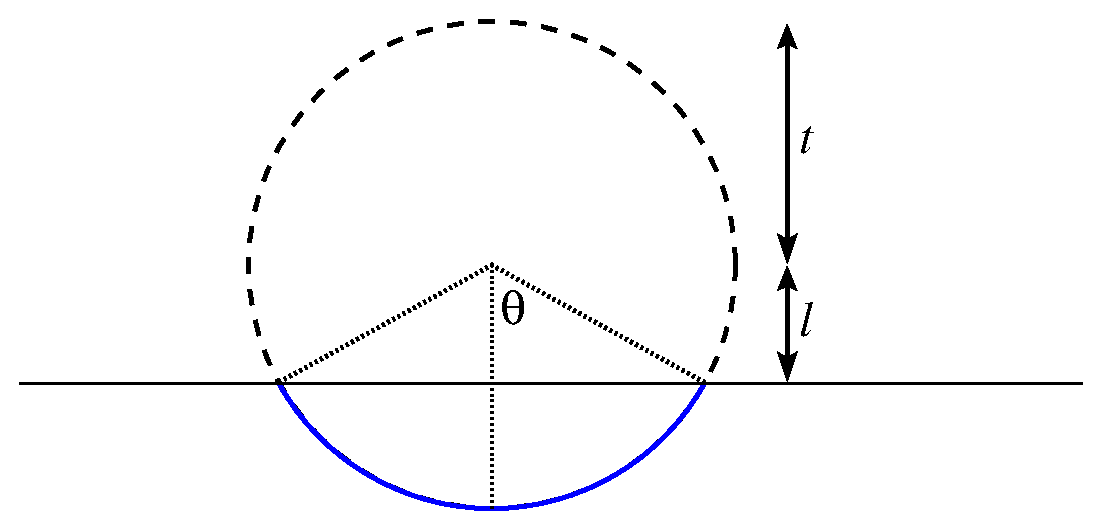
\includegraphics[width=0.33\columnwidth]{Figs/perimeter.eps}
    \caption{.}
    \label{fig:perimeter}
  \end{center} 
\vspace{-4mm}
\end{figure}

The next order correction would then build in the fact that the border
is not straight, e.g., in the case of a disk it is round, and in the
case of the square it has corners. However, as this term is very
dependent on shape and not general characteristics we won't calculate
it here.




\subsubsection{3D case}

Likewise for a region of 3D Euclidean space, we look at the
probability that the point lies on the surface of a sphere of radius
$t$, i.e.,
\begin{equation}
  g(t) \sim \frac{4 \pi}{V} t^2, 
\end{equation}
We can naturally generalize to $n$-D Euclidean spaces, by noting that
the generalized surface are of the $n$-D hyperball is
\begin{equation}
  \label{eq:surface_hyperball}
  S_{n} = \frac{dV_n}{dR} = n C_n R^{n-1}.
\end{equation}
where $V_n$ is its volume, and $C_n$ is defined in \eqref{eqn:cn}, so
the first order term of any expansion (for small $t$) of the density
function will take the form
\begin{equation}
  g(t) \sim \frac{n C_n}{V} t^{n-1}, 
\end{equation}
where $V$ is the $n$-D volume of the region of interest.

However, calculating the integral for the next term (correcting for
the perimeter would be tiresome, and in any case will be derived below.

\subsubsection{Higher dimensions}

We can go through exactly the same process in higher dimensions, to
obtain the same types of approximations, but computing the integrals
is somewhat redundant as we can see the correct forms of
approximatiosn directly from the hyperball distribution. Intuitively,
in high dimensions, the points are spread ``more thinly'' in the sense
that their density on $n$-dimensional volumes will be lower, and
hence, the distances between points will be larger. In particular the
chance of very short lines decreases, and we see this in the fact that
the first non-zero term in the Taylor series above has order $n-1$ for
the $n$-dimensional problem.

By the previous argument, we know that the result for the ball should
extend to arbitrary shapes, where $S_n$ is the general form of the
surface area, and $V_n$ the arbitrary form for the volume, so we could
for instance estimate the formula for small $t$ for a 4-rectangle with
sizes $a,b,c$ and $d$ as
\begin{eqnarray}
  g^{4D-{\rm rectangle}}_{a,b,c,d}(t)
 & \simeq  & 
      \frac{n C_n}{V_n} t^{n-1}
    -  \frac{ \pi^{(n-1)/2} }{\Gamma((n+1)/2)}
        \frac{S_n}{ V_n^2} t^{n} \nonumber \\
 & \simeq  & 
      \frac{2 \pi^{2}}{ a b c d} t^{3}
      -  \frac{8 \pi(abc + a b d + a c d + b c d)}{ 3 (a b c d)^2} t^{4}.
\end{eqnarray}



%%%%%%%%%%%%%%%%%%%%%%%%%%%%%%%%%%%%%%%%%%%%%%%%%%%%%%%%%%%%%%%%%%5

\subsection{Non-Euclidean Problems}

We can extend some of this insight into other problems, for instance,
the {\em circle line picking} problem, where pairs of points are
chosen on a circle, but the lines cross the circle. Here, the
probability distribution for line length (with a unit circle) is
\cite{weisstein:_circle_line_picking}
% http://mathworld.wolfram.com/CircleLinePicking.html
\begin{equation}
  \label{eq:circle_line_picking}
  g(t) = \frac{1}{\pi} \left(    
           1 - \frac{s^2}{4}
               \right)^{-1/2} 
       \simeq \frac{1}{\pi} \left( 1 - \frac{s^2}{4} + \cdots \right) 
\end{equation}
whereas in {\em sphere line
  picking}~\cite{weisstein:_sphere_line_picking}, there distribution
takes the form
\begin{equation}
  \label{eq:sphere_line_picking_approx}
  g(t) = \frac{1}{2} t.
\end{equation}
Clearly in this type of case, the dimension of the space is not the
critical factor, because the space on which the points are chosen is
embedded in a larger space from which lines are chosen, and the
geometry of the relationship is important.


INCIDENTALLY -- limit n -> infty for balls, has almost fixed distances
between nodes, so it approaches ER graph





\clearpage
\section{Numerical Computation by Simulation}
\label{sec:numerical}

It may be possible that one wishes to compute distributions, on
irregular regions, for which there is no closed form solution.
Numerically it is straight-forward to calculate the function
$g(t)$. There are two obvious approaches:
\begin{itemize}

\item Numerical computation of a $n$-dimensional integral over
  $\Omega$, or

\item Simulation of the problem, and estimation of the density from
  simulated results. 

\end{itemize}
The two approaches have different advantages and disadvantages. The
former approach has no stochastic component, and so errors are
predictable and regular. 

The later approach allows complex, potentially non-convex,
non-uniform, problems to be solved as long as they can be
simulated. Given the stochastic nature of the latter, it may help to
say a little more:

The general process is as follows:
\begin{enumerate}

\item Simulate a set of $2N$ points in the region of interest, and
  calculate the distances between successive pairs. The region may be
  irregular, or even non-convex; decisions may be made about some
  lines being inadmissable (because, for instance, they are exterior
  to the region for a non-convex region), or distances may be
  non-Euclidean, or the point distribution can be non-uniform. All
  that is needed is a set of output distances $\{ t_i \}_{i=1}^{N}$.

\item The density could then be approximate through binning, or a
  kernal smoothing technique, but in fact, we don't need direct access
  to the density as the estimator uses the Laplace transform.

\end{enumerate}

We have tested the above approach, running it 30 times (with different
seeds), in Matlab for various values of $N$. The results are shown in
Figure~\ref{fig:simulated_laplace}. The first plot shows estimates of
the mean relative absolute error of the estimated Laplace transforms
over the range $S \in [0, 50]$. We can see from the fitted straight
line, that the errors decrease as $1/\sqrt{N}$, dropping to around 1\%
at around $N=100,000$.


....





The second plot shows the computation times\footnote{Both algorithms
  were implemented in Matlab, the exact method using Matlab's {\tt
    quadqk} function. } relative to the computation times for the
``exact'' method\footnote{Note that both techniques are in some
  respect numerical, because even when we have a closed form solution
  for the density, we still typically need to numerically integrate
  this to obtain the Laplace transform, but we shall refer to this
  solution as ``exact'' for the sake of clarity in the following
  results, and because in the following we perform numerical
  integration with error tolerances of $10^{-6}$, which means the
  errors in this approach are significantly smaller than those of the
  simulation-based approach, at least for the ranges of $N$ tested
  here.}  We can immediately notice that computation times are roughly
linear in $N$, as one might expect. that around the range $N=100,000$,
the simulation approach is competitive with the exact approach.

The simulation-based approach is not as accurate as the exact
numerical approach, however, it accuracy should be sufficient for most
estimation problems, without increasing the computational workload
unduly.
make



\begin{figure}[tbp]
  \begin{center}
    \subfloat[line]{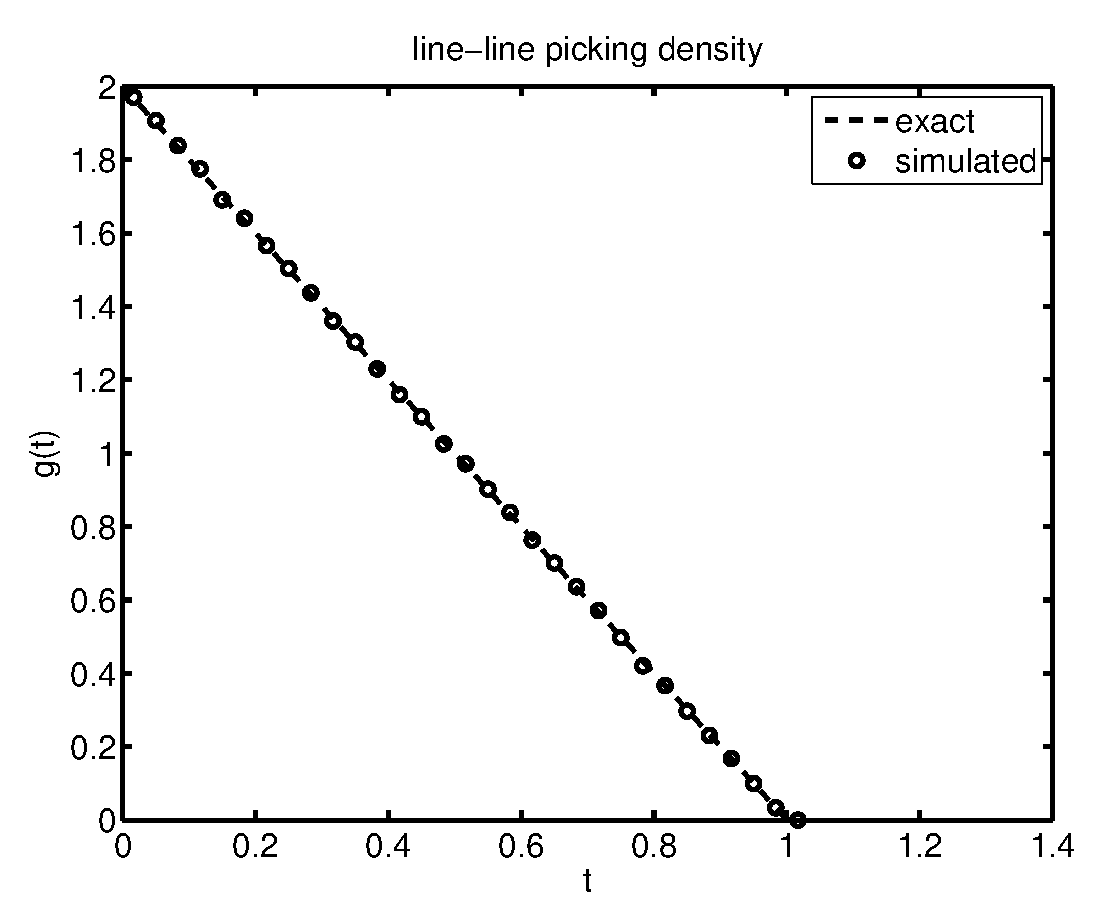
\includegraphics[width=0.32\columnwidth]{../Matlab/Plots/LinePicking_test_sim_line.eps}} 
    \subfloat[square]{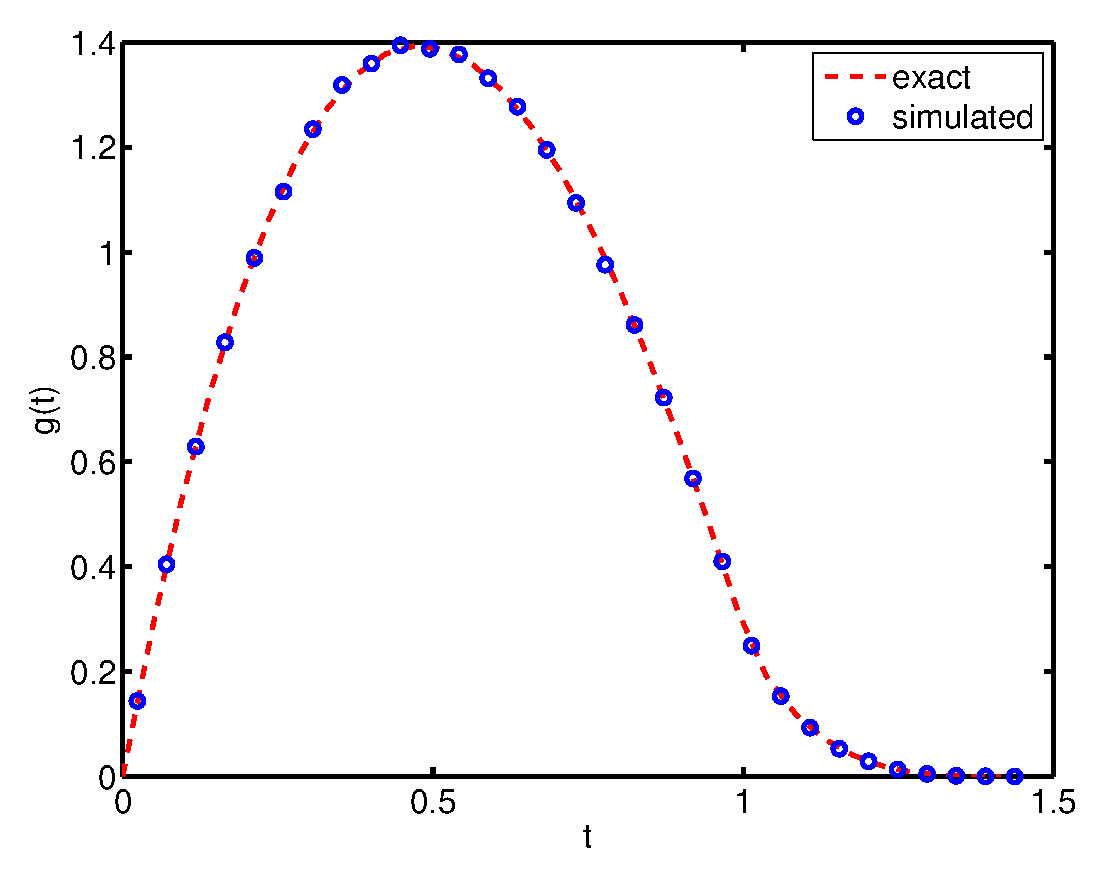
\includegraphics[width=0.32\columnwidth]{../Matlab/Plots/LinePicking_test_sim_square.eps}} 
    \subfloat[rect]{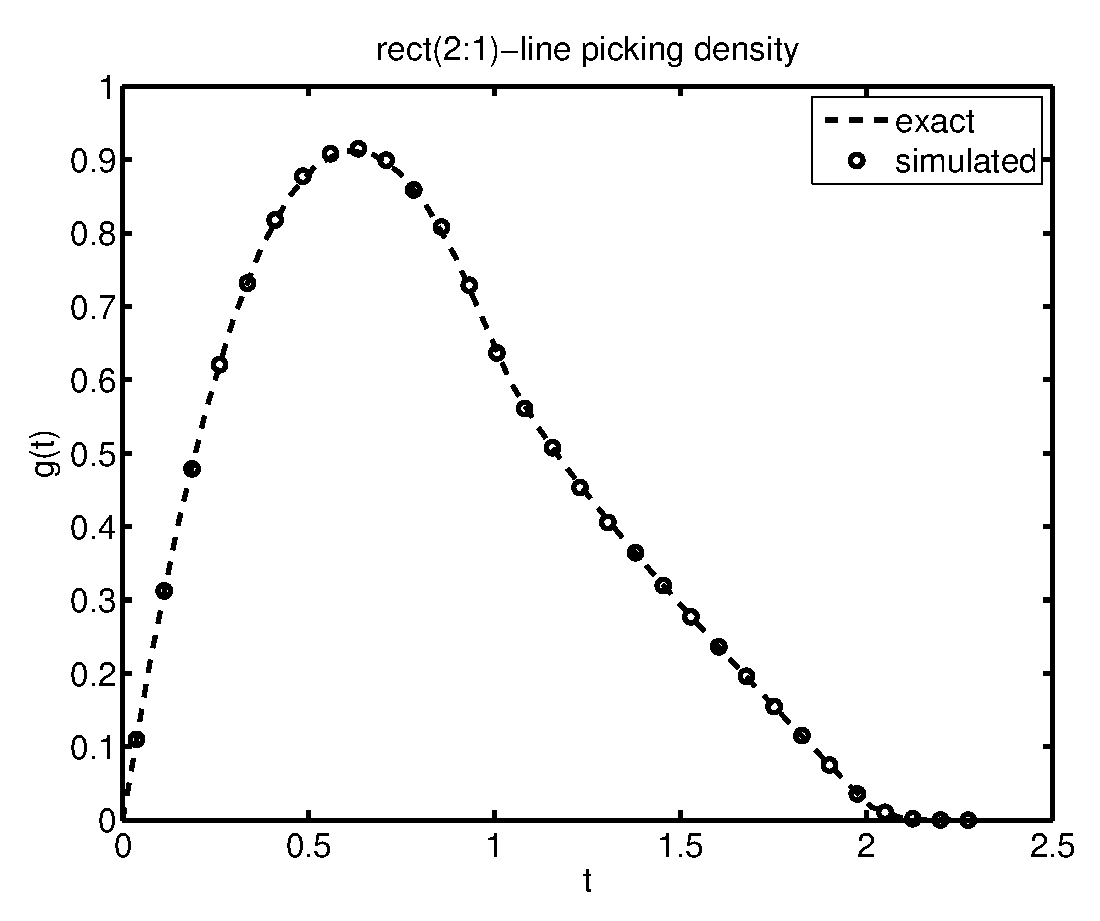
\includegraphics[width=0.32\columnwidth]{../Matlab/Plots/LinePicking_test_sim_rect.eps}} 

    \subfloat[cube]{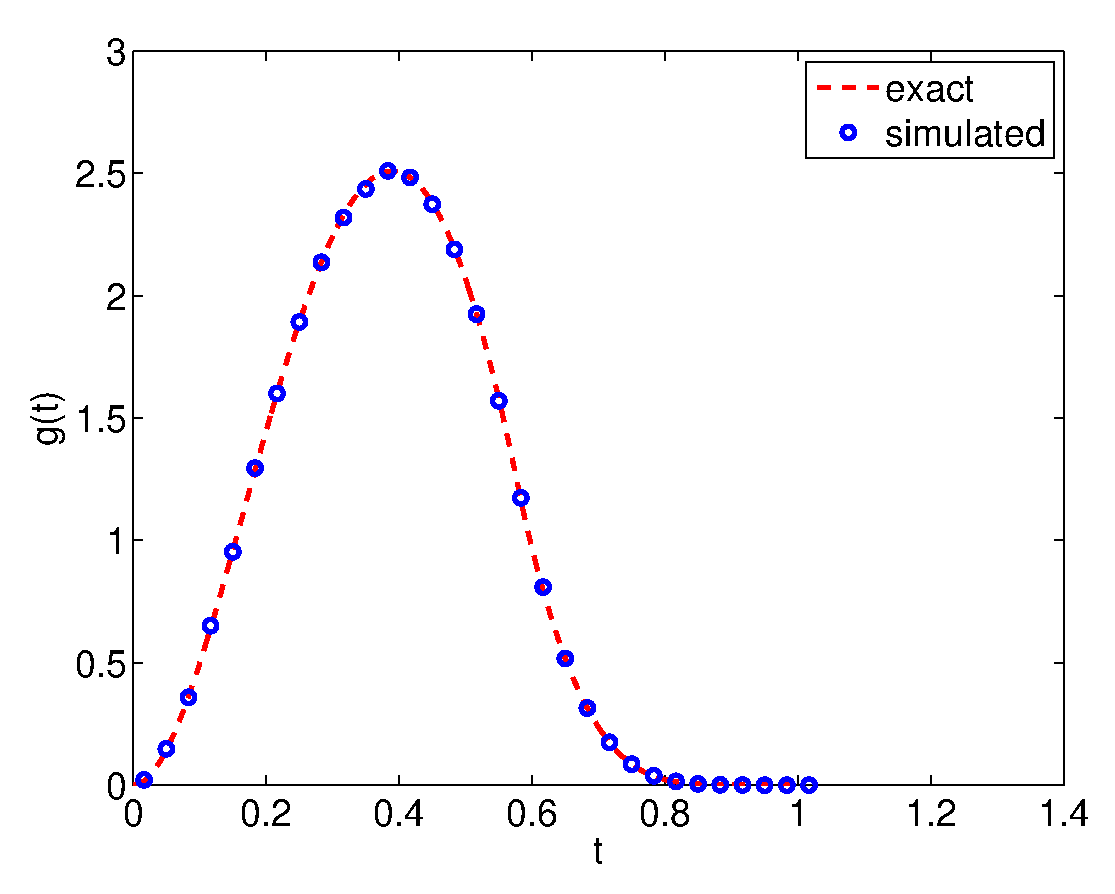
\includegraphics[width=0.32\columnwidth]{../Matlab/Plots/LinePicking_test_sim_cube.eps}} 
    \subfloat[3ball]{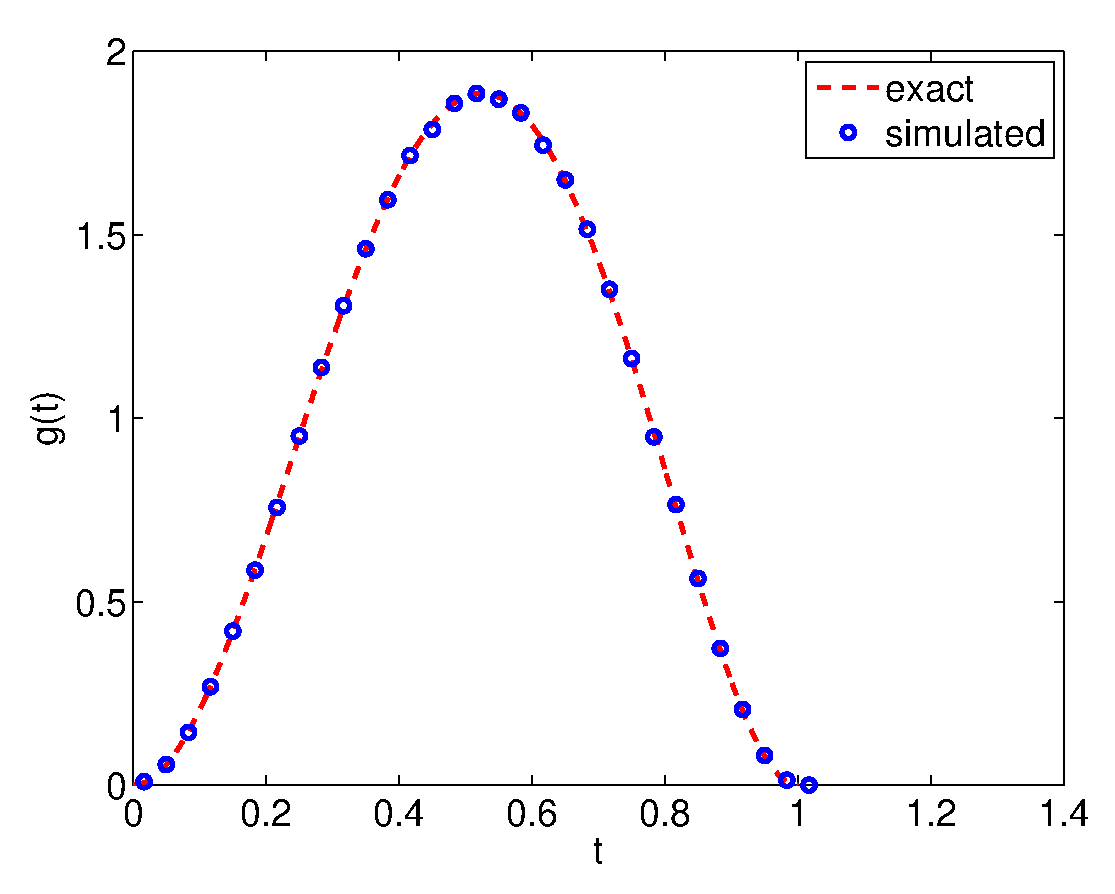
\includegraphics[width=0.32\columnwidth]{../Matlab/Plots/LinePicking_test_sim_3ball.eps}} 
    \subfloat[4ball]{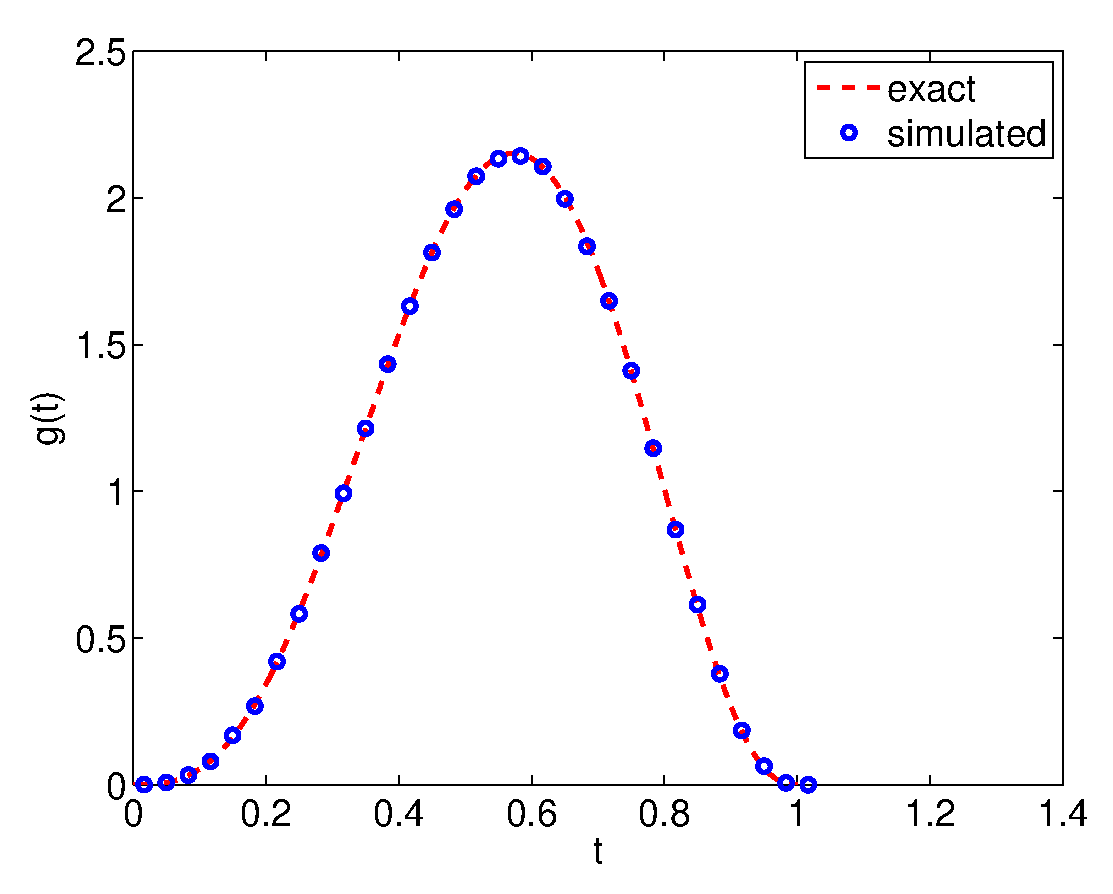
\includegraphics[width=0.32\columnwidth]{../Matlab/Plots/LinePicking_test_sim_4ball.eps}} 

    \subfloat[sphere]{\includegraphics[width=0.32\columnwidth]{../Matlab/Plots/LinePicking_test_sim_sphere.eps}} 
    \subfloat[sphere geodesic]{\includegraphics[width=0.32\columnwidth]{../Matlab/Plots/LinePicking_test_sim_sphere_geodesic.eps}} 
 

    \caption{\label{fig:sim_vs_exact}Comparisons of exactly calculated
      distributions and the distributions obtained by simulation. One
      million simulated lines were used to draw the estimated PDF,
      which are binned into 30 equally spaced bins.}
  \end{center} 
\vspace{-4mm}
\end{figure}



TABLE from \verb|LinePicking_test_sim|

  \begin{table}[ht]
    \centering
    \begin{tabular}{r|rrrr}
             problem &     mean & estimated mean & variance &  estimated var \\
     \hline 
              square &   0.5214 &         0.5214 &   0.0615 &         0.0615 \\
                disk &   0.9054 &         0.9060 &   0.1802 &         0.1804 \\
        3d hyperball &   1.0286 &         1.0278 &   0.1420 &         0.1421 \\
       1:2 rectangle &   0.8048 &         0.8050 &   0.1857 &         0.1855 \\
                line &   0.3333 &         0.3329 &   0.0556 &         0.0555 \\
                cube &   0.6617 &         0.6613 &   0.0621 &         0.0622 \\
              sphere &   1.3333 &         1.3332 &   0.2222 &         0.2221 \\
    \end{tabular}
    \caption{Means and variances calculated exactly, and approximated by simulation.}
    \label{tab:mean_var_estimates}
  \end{table}
% probably want parameters in the table ...

\clearpage
\section{Programs}
\label{sec:program}

\subsection{A Rough Guide}

The code is arranged to be usable as
\begin{enumerate}

\item Directly, as a command-line function;

\item By linking into a larger set of code;

\item Called through a {\tt Matlab} MEX wrapper; or 

\item Called through a {\tt R} wrapper function.

\end{enumerate}
It is designed to be as independent of external libraries as possible,
needing only the C standard libraries. So compilation should be
straight forward on the majority of machines.

Ideally, typing {\tt make} in the top level directory should make all
of the targets, however, {\tt R} users may find it easier to install
using standard {\tt R} installation procedures (but not that these
won't necessarily construct the other components, need for instance
for Matlab).

The makefiles in the subdirectories are named {\tt gMakefile} to avoid
conflicts with the way {\tt R} interprets them, so if you wish to
remake a specific subdirectory, enter the directory and type: 
\verb|make -f gMakefile|.

There are a large number of functions defined in the code, for each of
the cases discussed above, however, there are a small set of functions
that you may need to be aware of, that allow one to call all of the
others through a simple, uniform interface.

....


\subsection{Numerical Issues}

Most of the computations in the code involve simple calculations, with
no obvious numerical issues (other than the obvious fact that floating
point arithmetic is being used).

The computations on the $n$-D ball, however, require calculation of
the incomplete beta function. We have provided a separate library to
perform this computation, but users may find they can obtain more
accurate results using third party library functions. 

...

Estimates of errors ...


\subsection{Tests}

The tools come with a set of tests to compare performance on your
system with ours, and ensure everything is working ...




\clearpage
\section{Correlations}

Correlations between distances \cite{bartlett64}

(0) correlation between a pair 1/10

(i) $n$ nodes, then $N = n (n-1)/2$ pairs of nodes, and so this many pairs of distances

(ii) the $N (N-1) /2 = n (n-1) (n (n-1) -1)/8 = $ possible pairs of
correlations

(iii) but only $n(n-1)(n-2)/2$ of the correlations are positive,
because they share a node so we get average correlation between all
pairs
 \[ \frac{1}{10} \frac{n(n-1)(n-2)/2}{n (n-1) (n (n-1) -1)/8} =
    \frac{2}{5} \frac{(n-2)}{(n (n-1) -1)}
   \simeq 
   \frac{2}{5n}
\]
for large $n$

Empirical measurement (see triples.m)
\[ r = 0.114865 \pm 0.000037\]
 
 

 
\clearpage
\section{Conclusion and Future Work}


limit n large for various spherical cases

  -- approach Gaussian, distances are farish apart

  -- use to model distances between images

If distances are all similar as they seem to be, then Waxman
approaches ER graph 

\appendix 

\clearpage
\section{Useful definitions, functions and results}
\label{sec:useful}

This section covers some basic definitions, and results needed to make
this paper precise and self-contained.

Definitions:
\begin{description}

\item[PDF:] 

\item[CDF:]

\item[Support:]

\end{description}


Transformation of PDFs
If $y = g(X)$

\[ f_Y(y) = \left| \frac{d}{dy} \left( g^{-1}(y) \right) \right|
               f_X\left( g^{-1}(y) \right)
\]


\begin{eqnarray}
 E[ g(X) ] & = & \int y f_g (y) \, dy \\
           & = & \int g(x) f_X(x) \, dx 
\end{eqnarray}




\subsection{$\Gamma$ functions}

Definitions ...


where the Gamma function satisfies\cite[6.1.12]{Abramowitz_and_Stegun}
\begin{eqnarray}
 \label{eq:gamma}
 \Gamma(1/2) & = & \pi^{1/2}, \\
 \Gamma(3/2) & = & \frac{1}{2} \pi^{1/2}, \\
 \Gamma(k+1) & = & k!, \\
 \Gamma(k+1/2) & = & \frac{(2k)! \pi^{1/2}}{2^{2k} k!},
\end{eqnarray}



From ????
\begin{eqnarray}
  \int_0^{\pi} \sin^i(x) \, dx
    & = & \left\{ \begin{array}{ll}
        \displaystyle
      \frac{\sqrt{\pi} \Gamma\big( n/2 + 1/2 \big)}{\Gamma\big( n/2+1 \big)}.
      & \mbox{ for } i = 2k, \\
        \displaystyle
      \frac{\sqrt{\pi} \Gamma\big( n/2 + 1/2 \big)}{\Gamma\big( n/2+1 \big)}.
      & \mbox{ for } i = 2k+1, \\
           \end{array} \right. \nonumber \\
\end{eqnarray}



C standard library has routines

\subsection{$\beta$ functions}

The {\em beta function} and {\em incomplete beta function} are defined
to be 
\begin{eqnarray}
  \label{eqn:beta}
  B(p,q)    & = & \int_0^1 t^{p-1} (1 - t)^{q-1} \, dt = \frac{\Gamma(p) \Gamma(q)}{\Gamma(p+q)}, \\
  \label{eqn:beta_inc}
  B(x; p,q) & = & \int_0^x t^{p-1} (1 - t)^{q-1} \, dt.
\end{eqnarray}
From these, we define the {\em regularized beta function}
\begin{equation}
  \label{eqn:beta_reg}
   I(x; p,q) = \frac{ B(x; p,q)}{B(p,q)}.
\end{equation}

There are many results known for these functions. The few needed here
on a regular basis are given below:
\begin{eqnarray}
  I(x; p, q) & = & 1 - I(1-x; q, p) \hspace{7mm} \mbox{ from \cite{}}, \\
  I(x; p, q) & = &              
\frac{x^a (1-x)^b}{a B(a,b)}  \left\{ 
               1 +
               \sum_{i=0}^{\infty} \frac{B(a+1,i+1)}{B(a+b,i+1)} (1-x)^{i+1}
           \right\} 
     \hspace{7mm} \mbox{ from \cite[26.5.4]{Abramowitz_and_Stegun}}, \\
\end{eqnarray}
 

Beta functions need to be calculated for a number of the PDFs and CDFs
given in this work. The simple beta function can be computed using the
C-standard libraries $\Gamma$-function. There are also many libraries
which can calculate incomplete beta functions, however, in order that
this code be as self-contained as possible, we implement our own beta
function calculation based on the continued fraction approximation
described in \cite{}.


\subsection{Hypergoemetric functions}


\subsection{Elliptic integrals}



\subsection{$n$-balls and $n$-spheres}

Definitions

....


The generalized volume and surface area of an $n$-ball are given by:
\begin{eqnarray}
V_n(R) & = & C_n R^n,
 \label{eq:gen_vol} \\
S_{n-1}(R) & = & \frac{dV_n}{dR} = n C_n R^{n-1}.
 \label{eq:gen_surf}
\end{eqnarray}
where
\begin{equation}
 \label{eq:cn}
  C_n = \frac{ \pi^{n/2} }{\Gamma(n/2 + 1)}.
\end{equation}



 

\setlength{\parskip}{1mm}
\bibliographystyle{ieeetr}
% \bibliography{queueing_theory,books,ip_traffic,time_series,reliability,tcp,ospf,lrd,worms,internet,routing,bgp,topology,network,traffic_engineering,algorithms,optimization,history,graph}
\bibliography{LinePicking}

\end{document}


